%%%%%%%%%%%%%%%%%%%%%%%
% EIHW (ENGLISH) Thesis template 
%%%%%%%%%%%%%%%%%%%%%%%

%
%%% 20.06.2018- Alice Baird - alice.baird@informatik.uni-augsburg.de
%
%\documentclass[a4paper, 10pt, draft]{report}
\documentclass[a4paper, 11pt]{report}

\usepackage{ifdraft}

\usepackage{sectsty}
\chapternumberfont{\normalsize}
\chaptertitlefont{\normalsize}
% \chapternumberfont{\Large}
% \chaptertitlefont{\Large}

%\usepackage[showframe]{geometry}

\usepackage{psfrag,amsbsy,graphics,float}
\usepackage{verbatim}
\usepackage{url}
%\usepackage{cite}

\usepackage{wrapfig}
\usepackage[T1]{fontenc}
\usepackage[utf8]{inputenc}

\usepackage[active]{srcltx}
\usepackage{algorithm}
\usepackage[noend]{algorithmic}
\usepackage{amsmath}
\DeclareMathOperator*{\argmax}{arg\,max}
\DeclareMathOperator*{\argmin}{arg\,min}
\usepackage{amssymb}
\usepackage{amsfonts}
\usepackage{mathtools}
\usepackage{amsthm}
\usepackage{bbm}
\usepackage{enumerate}
\usepackage{graphicx}
\usepackage{ifthen}
\usepackage{listings}
\usepackage{struktex}
% \usepackage{hyperref} Do not hide links for final version!
\usepackage[hidelinks]{hyperref}
\usepackage{color}

\usepackage[english]{babel}
\usepackage{csquotes}
\usepackage[backend=biber,style=trad-abbrv]{biblatex}
\addbibresource{bib/speech-separation.bib}

% Define length
\setlength{\textwidth}{15cm}
\setlength{\textheight}{22cm}
\setlength{\evensidemargin}{-2mm}
\setlength{\oddsidemargin}{11mm}
\setlength{\topmargin}{10mm}
\setlength{\parindent}{0pt}

\usepackage{tabularx}
\usepackage{booktabs}

\usepackage[acronym]{glossaries}
\usepackage{pgf}
\usepackage[alsoload=binary]{siunitx}
\sisetup{binary-units=true}
% \usepackage{caption}

\makeglossaries

\newacronym{dft}{DFT}{Discrete Fourier Transform}
\newacronym{idft}{iDFT}{inverse Discrete Fourier Transform}
\newacronym{fft}{FFT}{Fast Fourier Transform}
\newacronym{ifft}{iFFT}{inverse Fast Fourier Transform}
\newacronym{stft}{STFT}{short-time Fourier Transform}
\newacronym{cola}{COLA}{constant-overlap-add}
\newacronym[longplural={Signal to Noise Ratios},shortplural={SNRs}]{snr}{SNR}{Signal to Noise Ratio}
\newacronym{srt}{SRT}{Speech Reception Threshold}
\newacronym[longplural={Deep Neural Networks},shortplural={DNNs}]{dnn}{DNN}{Deep Neural Network}
\newacronym[longplural={Recurrent Neural Networks},shortplural={RNNs}]{rnn}{RNN}{Recurrent Neural Network}
\newacronym{nmf}{NMF}{Non-negative Matrix Factorization}
\newacronym{ica}{ICA}{Independent Component Analysis}
\newacronym{isa}{ISA}{Independent Subspace Analysis}
\newacronym{dc}{DC}{Deep Clustering}
\newacronym{casa}{CASA}{Computational Auditory Scene Analysis}
\newacronym{ibm}{IBM}{Ideal Binary Mask}
\newacronym[longplural={Multilayer Perceptrons},shortplural={MLPs}]{mlp}{MLP}{Multilayer Perceptron}
\newacronym{mse}{MSE}{Mean Squared Error}
\newacronym{mae}{MAE}{Mean Absolute Error}
\newacronym{lstm}{LSTM}{Long Short-term Memory}
\newacronym{bptt}{BPTT}{Back-Propagation Through Time}
\newacronym{vad}{VAD}{Voice Activation Detection}
\newacronym{pca}{PCA}{Principal Component Analysis}
\newacronym{sphere}{SPHERE}{Speech Header Resources}
\newacronym{riff}{RIFF}{Resource Interchange File Format}
\newacronym{wce}{WCE}{Within Cluster Error}
\newacronym{gru}{GRU}{Gated Recurrent Unit}
\newglossaryentry{timit}
{
    name=TIMIT,
    description={Data set from Texas Instruments \& Massachusetts Institute of Technology}
}

\newglossaryentry{wsj0}
{
    name=WSJ0,
    description={Wall Street Journal Phase I Data set}
}
\newacronym[longplural={Source to Distortion Ratios},shortplural={SDRs}]{sdr}{SDR}{Source to Distortion Ratio}
\newacronym[longplural={Source to Interference Ratios},shortplural={SIRs}]{sir}{SIR}{Source to Interference Ratio}
\newacronym[longplural={Source to Artifact Ratios},shortplural={SARs}]{sar}{SAR}{Source to Artifact Ratio}
\newacronym[longplural={Image to Spatial Distortion Ratios},shortplural={ISRs}]{isr}{ISR}{Image to Spatial Distortion Ratio}

\usepackage{import}

\usepackage{tikz}
\usepackage{pgfplots}
\pgfplotsset{compat=1.16}
\usetikzlibrary{shapes,arrows,calc,positioning,fit,arrows.meta}

\theoremstyle{definition}
\newtheorem{definition}{Definition}[section]

\usepackage{multirow}

\usepackage{subcaption}
\usepackage[toc,page]{appendix}

%\usepackage{setspace}
%\doublespacing

\def\sigmoidfigure
{
    \begin{tikzpicture}[trim axis left, trim axis right, baseline]
        \begin{axis}[axis lines=none,width=2cm,height=2cm,
                ylabel shift=-0.1cm]
            \addplot[color=black]{1/(1+exp(-x))-2};
        \end{axis}
    \end{tikzpicture}
}

\def\tanhfigure
{
    \begin{tikzpicture}[trim axis left, trim axis right, baseline]
        \begin{axis}[axis lines=none,width=2cm,height=2cm,
                ylabel shift=-0.1cm]
            \addplot[color=black]{(exp(2*x) -1)/(exp(2*x) + 1)};
        \end{axis}
    \end{tikzpicture}
}


\tikzset{
    neuron/.style={circle,minimum size=29pt,inner sep=0pt, draw},
    input neuron/.style={neuron},
    output neuron/.style={neuron},
    hidden neuron/.style={neuron,fill=black!25},
    cell neuron/.style={neuron,fill=black!25},
}

% used to avoid putting the same thing several times...
% Command \empt{var1}{var2}
\newcommand{\empt}[2]{$#1^{\langle #2 \rangle}$}


% Math
\newcommand*{\doubletran}{^{\mkern-1.5mu\mathsf{T}^{\mkern-1.5mu\mathsf{T}}}}
\newcommand*{\tran}{^{\mkern-1.5mu\mathsf{T}}}
\newcommand*{\frob}{_{\mkern-1.5mu\mathsf{F}}} % Not used as alignment is off
\newcommand\numeq[1]%
  {\stackrel{\scriptscriptstyle#1}{=}}
\allowdisplaybreaks

% Typesetting
\clubpenalty=10000
\widowpenalty=10000

\usepackage{float}

\pdfsuppresswarningpagegroup=1

% Figure <-> Text
\setlength{\intextsep}{13pt plus 1.0pt minus 2.0pt}

\usepackage[titles]{tocloft}
\setlength{\cftbeforechapskip}{6pt}

\begin{document}
\pagestyle{empty}

\begin{titlepage}
	\centering
	% \hfill
\includegraphics[width=0.25\textwidth]{figure/Uni_Aug_Logo_Basis_pos_B}\par
	
\includegraphics[width=0.5\textwidth]{figure/Uni_Aug_Logo_Basis_pos_B}\par
	% 
\includegraphics[width=0.20\textwidth]{figure/Uni_Aug_Logo_Basis_pos_C.eps}\par
	\vspace{1cm}
	% {\scshape\LARGE University of Augsburg \par}
	{\scshape\large Chair of Embedded Intelligence for Health Care and Wellbeing \par}
	{Univ.-Prof. Dr.-Ing. habil. Bj{\"o}rn \textsc{Schuller} \par}
	\vspace{2.5cm}
	{\scshape\LARGE Bachelor Thesis \par}
	\vspace{1.0cm}
	{\Huge\bfseries Speech Separation using\\Deep Clustering \par}
	\vspace{3.0cm}
	{\Large Maximilian \textsc{Ammann} \par}
	{Matrikel-Nr.: 1471541 \par}
	\vfill

	supervised by Shuo \textsc{Liu}

	\vspace{2cm}

	% Bottom of the page
	{\large October 14, 2019\par}
\end{titlepage}

\topmargin5mm
\textheight220mm

\small

\begin{abstract}

	\begin{center}
		%\normalsize \textbf{Abstract}\\
	\end{center}

	% What is speech separation?
	Speech separation is the task of separating the voices of concurrently speaking persons.
	Compared to traditional signal processing approaches Deep Clustering presents a data-driven method which outperforms the classical ones.

	% DC and what are the key points of it
	In Deep Clustering, a recurrent neural network is trained to embed each time-frequency bin of a monaural speech spectrum into a high-dimensional space. The affinity of these embedding vectors in the target space is exploited to segment the spectrogram using k-means clustering. Vectors with low distance between each other belong to the same speaker. Therefore, the segmented clusters allow to create a spectrum mask for each speaker. Additionally, the mask is applied to the mixture in order to separate the voices. Finally, the time-domain speech signal is reconstructed.
	The approach offers speaker-independent separation and achieves an \acrlong{sdr} of 8.89 on the high fidelity TIMIT data set.

	% What was the goal of this thesis? Adaptability and Reproducability
	In the thesis, experiments were conducted to find out whether the evaluation results of the original Deep Clustering paper hold true for different data sets which were not recorded under laboratory conditions.
	Therefore, the algorithm has been evaluated on various data sets, namely WSJ0, TIMIT and the freely available TEDLIUM, in order to determine its adaptability to varying grades of quality.
	Furthermore, the thesis states the stages of Deep Clustering precisely and presents a free and open source implementation.

	% What are the findings?
	The findings include that the quality of separation suffers from noise in the training and evaluation data set. In contrast, unknown speakers do not affect the success to the same extent.
	These results illustrate how important the data set is, and hence more research is needed on preparing real-world data.

	% What was additionally done? Visualizations
	For this reason two methods for visualizing the embedding vectors were introduced. The first illustration uses the linear dependence between the vectors whereas the second selects different orders for clustering to draw a conclusion about the success of Deep Clustering.

\end{abstract}

\thispagestyle{empty}
\pagestyle{empty}
\pagenumbering{gobble}

\tableofcontents
\cleardoublepage

\pagenumbering{arabic}
\pagestyle{plain}

\addcontentsline{toc}{chapter}{Abbreviations}
\setglossarystyle{alttree}
\glssetwidest{xxxxxxxxx}
\printglossary[type=\acronymtype,title={Abbreviations},nonumberlist,nopostdot]
\cleardoublepage


%
%
% The content should be 30-40 pages including figure, but without title, ToC, appendix etc.
% Final TODO: Check usage of figure vs. Figure, section vs. Section
% Final TODO: Check~\textcite for singular vs. plural
% Final TODO: Make matrices/vectors bold
% Final TODO: Start at 0 or 1 -> Start at 0
% Final TODO: Check if transpose is correct for weights. Also check order of multiplication. One could also assume that weights are already transposed.
% Final TODO: Check Outline/Start,End of sections
%

\chapter{Introduction}
% Reference to Star Trek Dejavu?

The goal of source separation is to separate a mixture into estimated sources.
There have been many approaches to the task of separating signals in a variety of areas such as automated karaoke, object-specific equalizers, hearing prostheses and robust speech recognition~\cite{Wang2018}.
% TODO: More motivation and application
Algorithms can use assumptions whether or not the signal is stereo or whether certain harmonic or redundant compositions exist~\cite[p.~1308]{Rafii2018}.
% TODO: Difference to Lead and Accompaniment separation: No Harmonic and Redundant hints

% Cocktail-Party-Problem and human hearing
The domain discussed in this thesis is the separation of speech.
In 1953 the ''Cocktail Party Problem'' was coined by~\textcite{Cherry1953}. Even for humans it can be difficult to understand other speakers during a cocktail party due to the quantity of concurrently speaking people. In most cases though the impressive human auditory system is capable of understanding a single speaker among many others without problems.
\textcite{Miller1947,Rosen2013} experimentally showed that the problem of separating voices is difficult even for humans because of the similarity of spectral and temporal features. Separating speech from other kinds of noise like a high frequency tone presents a less challenging problem for humans~\cite[p.~128]{Miller1947}.

\begin{figure}[ht]
	\centering
	{
		\fontsize{8pt}{10pt}\selectfont
		\import{figure/}{figure/intelligibility.pdf_tex}
	}
	\caption{Speech intelligibility score for different kinds of noise (from~\cites[p.~2]{Wang2018b}[p.~7]{Wang2006}, redrawn from~\cite{Miller1947}). Complex tones are repetitive pulses of square waves with harmonically related frequencies. Broadband noise consists of randomly related frequencies over a broad spectrum. The properties of the 1, 2 and 8 voices signals are self-explanatory.
		The vertical dotted lines correspond to the -20, -10 and 3 \si{\dB} \glspl{srt}.}
	\label{fig.intelligibility}
\end{figure}

Figure~\ref{fig.intelligibility} shows the intelligibility for different kinds of noises with different \glspl{snr}. Speech inside a mixture with a 10-20 \si{\dB} more powerful complex tone noise or one additional voice is still about 50\% intelligible for humans.~\textcite{Wang2018b} mention the concept of \gls{srt} which can be seen in Figure \ref{fig.intelligibility} at the intersection point of the intelligible score for each signal and the dotted line, projected onto the \gls{snr} axis. For example the interference with one voice has a \gls{srt} of about -10\si{\dB}.
They also highlight that there is a 23\si{\dB} \gls{srt} difference between complex and broadband noise. This means that the ability of humans to understand voices when mixed with noise highly depends on the kind of noise.

\textcite{Miller1947} also concludes that even though interference with high frequency signals doesn't reduce intelligibility as much as with low frequency ones, they are considered to be more annoying. The same applies to irregular interference. However, there is no evidence that annoyance reduces the intelligibility scores.

Note that the mixtures in Figure \ref{fig.intelligibility} are played in a laboratory situation with a monaural setup~\cite{Miller1947}. As we focus on monaural speech separation, this evaluation gives a good impression of what we try to achieve with an algorithmic approach to the problem. We will not make use of the ''binaural advantage'' (multichannel advantage) mentioned in~\cite[p.~7]{Wang2006} in this thesis.

We can conclude that the separation of speech is not a trivial task for humans. Especially for hearing impaired individuals it can be even more challenging as the \gls{srt} can be expected to be 4-6 \si{\dB} lower~\cite{Festen1990}. The development of an algorithm to perform the separation is also non-trivial which will be shown in Chapter \ref{sec.approaches} by summarizing the history of speech separation and its milestones.

\section{Challenges in Speech Separation}\label{sec.challenges}
% Definition of the general problem
Speech separation is a challenging problem because there is not a single perfect solution.
Let $x_1(n_1)$ and $x_2(n_2)$ be the reference samples of two audio signals for $0 \le n_1 < N_1$ and $0 \le n_2 < N_2$, then the mixture signal is defined as $x = x_1 + x_2$ with the length $N = \min(N_1, N_2)$.
The goal of speech separation is to split the signal $x(n)$ into the target reference signals. Unfortunately, an infinite amount of solutions exists to this problem, because this is a highly underdetermined task.

% Blind source separation
This ambiguity is even more severe if the separation is conducted blind which means that no prior knowledge about the mixture is  available. This includes knowledge like the count, gender or age of the speakers.

% Speaker dependent vs independent
Speech separation is called to be speaker-dependent if the speakers have to be the same for training and testing. Target-dependent means that the dominant speaker has to be the same during training and testing. Speakers who cause interference can be chosen arbitrarily. The most difficult goal for an algorithm is to be speaker-independent, which means that the algorithm also performs well if the speakers during testing are completely unknown.~\cite[p.~15]{Wang2018b}

% Speech Enhancement is special case of speech separation
Speech enhancement can be seen as a special case of speech separation. % Missing cite
Enhancement means that a disturbing component of the audio should be removed. That component can be static noise, noise from cars or babble. Noise can be seen as an additional source in the context of speech separation. Nevertheless, it is often ignored in speech separation because the main goal is to get source estimations for speech.
Therefore, a field which naturally profits from advances in speech separation is speech enhancement. Another profiting field is automatic speech recognition~\cite{Qian2018}. A signal with exactly one speaker and less noise is a better input for speech recognition than a noisy one.

In this thesis we try to achieve blind speech separation. Music or powerful background noise it not expected during training and testing of the \gls{dc} model. This is still a difficult challenge because we try to separate sources within the same domain. The next chapter focuses on the methods which have been tried in the past.

\section{Earlier Approaches}\label{sec.approaches}
% More earlier approaches: https://pdfs.semanticscholar.org/c383/833d5083b9513f65e80d2dab6d8389e58b92.pdf

For the past 6 decades it is true that the ''Cocktail Party Problem'' hasn't been solved properly~\cite[p.~2]{Wang2018b}. Nevertheless, recently impressive progress has been achieved by using \glspl{dnn}. In this chapter we will go over earlier work and also cover the latest achievements in speech separation, which make use of \glspl{dnn}.

The earliest methods for achieving a separation of audio used digital signal processing techniques. In~\cite{Ephraim1985} speech enhancement was achieved by using estimators in the time-frequency domain. According to a subjective comparison in~\citeyear{Hu2007} this approach performs well compared to other methods proposed at that time~\cite{Hu2007}. It is noteworthy though, that all competing algorithms did not achieve to enhance the noisy audio significantly in the presence of multiple background speakers~\cite[p.~601]{Hu2007}.

\gls{casa} focuses on modeling the human auditory system in order to achieve goals like automatic speech and speaker recognition, music transcription, improving hearing prostheses or audio information retrieval~\cite[p.~13]{Wang2006}. Compared to the other approaches mentioned, \gls{casa} is driven by the motivation to model the human~\cite[p.~29]{Wang2006}. The other approaches are application-driven and focus on digital signal processing. An analogy for the difference between \gls{casa} and digital signal processing is given by the difference between computational vision and computer vision, where the former is concerned about modeling the human and the latter about practical processing~\cite{Marr1982}.
Approaches in the field of \gls{casa} use spectrum, pitch and model based methods to separate speech~\cite[p.~106]{Wang2006}.

Later approaches use \gls{ica} or its extension Independent Subspace Analysis~\cite{Dubnov2002,Casey2000} in order to perform blind source separation. \gls{ica} exploits the assumption that the source components are statistically independent.
The model of this source separation is $x = As$, where $A$ is a $n \times \rho$ invertible mixing matrix with linearly independent columns, $s=\begin{psmallmatrix}s_1 & s_2 & \ldots & s_{\rho}\end{psmallmatrix}\tran$ is a vector which contains the sources and $x=\begin{psmallmatrix}x_1 & x_2 & \ldots & x_{n}\end{psmallmatrix}\tran$ is a vector which describes the mixture, where $n \ge \rho$.
The unmixing matrix $W \approx A^{-1}$ is calculated using $x$ and the fact that the vectors in $s$ are statistically independent~\cite{Casey2000}. The estimated source signals are defined as $Wx$.
Several approaches exist in order to exploit this independence, but the model and assumptions are equal.
\textcite[p.~1067]{Virtanen2007} notes that \gls{ica} is applicable for multichannel blind source separation, but can't be directly applied to monaural signals. \gls{isa} does not require multichannel audio~\cite[p.~1067]{Virtanen2007}.

In~\citeyear{Virtanen2007},~\textcite[p.~1071]{Virtanen2007} achieved better separation performance than \gls{ica} and \gls{isa} using \gls{nmf}. \gls{nmf} approximately factorizes a non-negative matrix $V \in \mathbb{R}_+^{n \times m}$ into two non-negative matrices $W \in \mathbb{R}_+^{n \times \rho}$ and $H \in \mathbb{R}_+^{\rho \times m}$~\cite{Schuller2010,Lee1999}. In digital signal processing \gls{nmf} is used on the magnitude spectrum (see Equation \ref{eq.decibel}). Therefore, the constraint of non-negativity is not a problem because the magnitudes in the frequency representation are already positive. The mixture is seen as a linear combination of the components $W$ and $H$~\cite{Schuller2010}.
% More info: https://ieeexplore.ieee.org/document/5495567/references#references
In~\cite{Schmidt2006} a supervised learning approach is presented which makes use of personalized phoneme dictionaries to prepare $W$.

Models like \gls{nmf} and \gls{ica} are linear. Therefore,~\textcite{Huang2014} propose the use of more complex nonlinear \glspl{dnn} and \glspl{rnn} with the goal of modeling voices better in~\citeyear{Huang2014}. This work represents one of the earliest uses of \glspl{rnn} for speech separation.
Neural networks offer multiple nonlinear layers which already proved valuable in tasks like speech enhancement. % TODO: Cite: Recurrent neural networks for noise reduction in robust ASR, Schöller: https://hal.inria.fr/hal-01163493/document
The \gls{rnn} proposed in~\cite{Huang2014} takes for each time step $t$ the spectral features as input and outputs the concatenation of two estimated sources $\hat{y}_1^{(t)}$ and $\hat{y}_2^{(t)}$ as seen in Figure \ref{fig.huang.structure}. An additional step is needed such that the sum of the estimated sources is equal to the mixture.
A binary or soft time-frequency mask like defined in Definition \ref{def.ibm} must be computed from the estimated sources which can be element-wise multiplied with the mixture to get the final estimated sources.
%The binary mask is implemented as the last layer in the network.
The approach achieved a 3.8-4.9\si{\dB} improvement compared to \gls{nmf} on the TIMIT~\cite{Garofolo1993} data set. % https://sites.google.com/site/deeplearningsourceseparation/
Note that according to the definition in Section \ref{sec.challenges} this approach is not speaker independent as it uses the same speakers during training and evaluation.
\begin{figure}
	\centering
	\begin{tikzpicture}
    % Hidden cells
    % Empty rectangle
    \node[rectangle] (Y0) at (0, 0) {};
    \node[cell neuron, right=2em of Y0] (RNN) {\sigmoidfigure};
    % Empty rectangle
    \node[rectangle, right=2em of RNN] (RNNHIDDEN) {};

    % Input/Output neurons
    \node[input neuron, below=of RNN] (X1) {$x^{(t)}$};
    \node[output neuron, above left=of RNN] (Y2) {$\hat{y}_1^{(t)}$};
    \node[output neuron, above right=of RNN] (Y3) {$\hat{y}_2^{(t)}$};

    \node[rectangle, left=of Y2, text width=2.5cm] {Output Layer};
    \node[rectangle, left=of RNN, text width=2.5cm] {Hidden Layer};
    \node[rectangle, left=of X1, text width=2.5cm] {Input Layer};


    \draw[-stealth, thick] (X1) -- (RNN);
    \draw[-stealth, thick] (RNN) -- (Y2);
    \draw[-stealth, thick] (RNN) -- (Y3);

    %  Dotted arrows
    \draw[-stealth, thick, densely dotted] (Y0) -- (RNN);
    \draw[-stealth, densely dotted, thick] (RNN) -- (RNNHIDDEN);
\end{tikzpicture}
	\caption{Structure of the layers in the \gls{rnn} from~\cite{Huang2014}. The spectra for two speakers $\hat{y}_1^{(t)}$ and $\hat{y}_2^{(t)}$ is estimated at time step $t$. The input spectrum $x^{(t)}$ is the mixture with both speakers.}
	\label{fig.huang.structure}
\end{figure}

Instead of defining an \gls{ibm}, it is also possible to use the calculated magnitude spectra directly like proposed in~\cite{Tu2014}.~\textcite{Qian2018} argue that the direct estimation of the spectrum is inferior because masks are more robust to changes of the input signals visible in the power spectrum.
% Maybe-TODO: 1-2 more approaches like CNNs, GANs: Wang2018b

A constraint of the so far mentioned deep learning approaches is that they are only able to separate $k$ speakers when trained on $k$ speakers. By introducing the \gls{dc} method we will try to overcome this limitation.

\label{sec.challenges.label-permutation}
Furthermore, the mentioned spectra and mask based methods suffer from the label ambiguity or permutation problem, which prevented progress for several years.
The problem is that if the spectra or masks are calculated using a \gls{dnn} like shown in Figure \ref{fig.huang.structure}, it is unknown which of the estimated spectra $\hat{y}_1^{(t)}$ and $\hat{y}_2^{(t)}$ belongs to which speaker. It is not easily possible to specify that $\hat{y}_1^{(t)}$ always corresponds to the same speaker as the permutation of the spectra should be a different for the next time step $t+1$. A naive approach to this problem would be to train the network that the first spectrum should always be the female speaker. This fails though if there are more speakers or same gender speakers are considered.~\cite[p.~4]{Kolbaek2017}

%TODO: Add more challanges of speech separation

As we will see \gls{dc} represents a state-of-the-art solution for speech separation. We will explore this approach in full detail to prove this statement in this thesis. The next section gives an outline of the whole thesis before we start to define \gls{dc} properly.

\section{Outline}

The findings of this thesis include that the speech separation using \acrlong{dc}:

\begin{itemize}
	\item allows to visualize the clustering and separation process
	\item and is speaker-independent,
	\item but suffers from noise in the training and evaluation data sets.
\end{itemize}

In order to make these contributions the thesis is structured in the following way.
The first chapter focused on the motivation, idea and challenges behind speech separation. It also introduced the classical approaches to speech separation.

The second chapter covers the foundations for \gls{dc} by discussing the discrete Fourier transform, deep neural networks (specifically recurrent neural networks) and k-means clustering.

The main chapter goes in detail about the state-of-the-art \gls{dc} approach. We go over the aspects of \gls{dc} in detail by splitting the method in several stages. The foundations of the previous chapter are used to describe the process of separation speech.

Chapter~\ref{sec.experimental-evaluation} focuses on an experimental evaluation of the implemented model. Visualizations of the clustering are presented by using \gls{pca} and order selection in the sections \ref{fig.clustering-pca} and \ref{sec.order-selection} respectively. The constrains of the evaluation environment are described in detail to make the results reproducible. Practical methods are explained and evaluation results given.

Finally, a conclusion about the adaptability of deep clustering to real-world data is drawn.

\chapter{Foundations of Deep Clustering}

As the \gls{dc} approach consists of several stages like described in Chapter \ref{chapter.dc} several topics should be covered in order to provide a deeper understanding of the applied method.
The following three sections provide the foundations for \gls{dc} by introducing the discrete Fourier transform, neural networks and k-means clustering.

\section{Discrete Fourier Transform}\label{sec.foundation-dsp}

% Samples, sample size, amount of samples, sample rate

Signal processing has two categories, one of which is analog signal processing. Its objective is to process signals which are continuous in time. The other one is digital signal processing which processes discrete signals and is used throughout this thesis.
A discrete signal is not a continuous waveform but a sequence of discrete values, where value corresponds to a time step.~\cite[p.~2]{Lyons1997}

In the context of digital audio a signal has a length $N$ which corresponds to the amount of samples. Furthermore, there is also the sample rate which is defined as the amount of samples per second. As we are dealing with digital data each sample also has a sample size in bit and a data type. Therefore, a discrete audio signal can be characterized by Table \ref{table.example.characteristics}.

\begin{table}
	\centering
	\begin{tabularx}{.6\textwidth}{lcl}
		Characteristic    & Symbol & Example\tabularnewline
		\midrule
		Amount of samples & $N$    & $16000$\tabularnewline
		\midrule
		Sample rate       & $f_s$  & $\SI{8}{\kHz}$\tabularnewline
		\midrule
		Sample size       & -      & $\SI{16}{\bit}$\tabularnewline
		\midrule
		Sample data type  & -      & Float (Little-endian)\tabularnewline
	\end{tabularx}
	\caption{Characteristics of an example discrete signal.}
	\label{table.example.characteristics}
\end{table}

The analysis, manipulation and synthesis of digital audio signals often requires to transform the signal to the frequency-domain. The \gls{dft} is a mathematical procedure which determines the frequency content of a discrete signal. The \gls{dft} $X(m)$ of the time-domain signal $x(n)$ is defined as

\begin{equation}
	X(m) = \sum_{n=0}^{N-1} x(n)e^{-i2\pi n m / N},
	\label{eq.dft}
\end{equation}
% Not to be confused with: Discrete-time Fourier transform
% Numpy implementation: https://docs.scipy.org/doc/numpy/reference/routines.fft.html#module-numpy.fft

where $m$ is the index of the frequency bin, $N$ is the amount of samples, $e$ is the base of the natural logarithm and $i$ the imaginary number~\cite[p.~49-50]{Lyons1997}.
The Fourier transform is a cornerstone in the analysis of signals and is used in a lot of fields. An infamous quote of William Thomson explains that ''Fourier's Theorem is not only one of the most beautiful results of modern analysis, but it is said to furnish an indispensable instrument in the treatment of nearly every recondite question in modern physics''.

% Symmetry
If $x(n)$ is a real valued signal, which means that the imaginary part is assumed to be zero, the \gls{dft} is symmetric. For simplicity, we assume that $N$ is even as this will also be the case in the application of \gls{dc}.
For $m=0$ to $m=\frac{N}{2}$ the result of $X(m)$ is redundant to the values for $m>\frac{N}{2}$. Thus for $0 \le m < N$ the magnitudes $|X(m)|$ and $|X(N-m)|$ are equal~\cite[p.~63]{Lyons1997}.

% Scaling and resolution
The non-redundant complex output of the \gls{dft} are $\frac{N}{2}+1$ values which are called frequency bins.
Unfortunately, the bins provide no information about the time interval in which the samples were taken. In order to scale the frequency bins according to an absolute frequency axis we need to scale the indices $m$ by $\frac{f_s}{N}$. For example, if $f_s=\si{\kHz}$ and $N=16k$ then the frequency bin with an index of one corresponds to a frequency of $f=\si{\kHz}$~\cite[p.~67]{Lyons1997}.
This scale allows determining dominant frequencies in the defined time interval.
The maximum frequency in this case is $\frac{N}{2}\frac{f_s}{N}=\frac{f_s}{2}$ which is also known as the folding or Nyquist frequency~\cite[p.~28]{Lyons1997}.
The first bin with $m=0$ is also called the DC (direct current) bias and represents the mean of the input and can therefore be ignored in the analysis of the signal~\cite[p.~15]{Heinzel2002}. The last bin $m=\frac{N}{2}$ can also be ignored because anti-aliasing filters should have removed the corresponding frequencies~\cite[p.~16]{Heinzel2002}.
The frequency resolution of the \gls{dft} is limited by the sample count within the time interval.~\cite[p.~51]{Lyons1997}

Another property of the \gls{dft} as defined by~\textcite[p.~65]{Lyons1997} is linearity. If $x_1(t)$ and $x_2(t)$ are discrete signals and $X_1(t)$ and $X_2(t)$ their corresponding transforms then the \gls{dft} of the sum $x_{sum}(t)=x_1(t)+x_2(t)$ is $X_{sum}(t)=X_1(t)+X_2(t)$.
The goal of source separation is to separate a signal like $x_{sum}(t)$ into its sources like defined at the beginning of the chapter.
Because of the linearity of the \gls{dft}, it is possible to perform the separation in the frequency-domain as done in the deep clustering approach (see Section \ref{sec.preprocessing} and \ref{sec.reconstruction}).

% Squared spectrum representation
For analysis of speech we are interested in the power instead of the magnitudes which is defined as $X_{pwr}(m)=|X(m)|^2$. So the magnitudes of the signal are proportional to its power~\cite[p.~9]{Lyons1997}. A useful unit for the power spectrum is dB (decibel). The conversion from a linear power spectrum to a logarithmic one is defined as
\begin{equation}
	X_{dB}(m)=10\log_{10}(|X(m)|^2)\,\si{\dB}=20\log_{10}(|X(m)|)\,\si{\dB}.
	\label{eq.decibel}
\end{equation}
Using the decimal logarithm has an advantage when evaluating power differences. It allows greater resolution when the power levels are small~\cite[p.~487]{Lyons1997}.

% Role of windows
An effect which needs to be acknowledged is leakage. Leakage causes the results in the frequency-domain to be only an approximation to the originals signals before sampling. Frequencies which are not exactly centered in a frequency bin are spread over all other bins~\cite[p.~71]{Lyons1997}. In order to reduce this effect windows can be used~\cite[p.~80]{Lyons1997}. Instead of using a rectangular window, which is equal to using no window, a window like the Hann window can be used. Amplitudes in a time interval multiplied by this window are near zero in the begging and the end. An example for a window like this be seen in Figure \ref{fig.hann}. This window will be used throughout this paper.
\begin{figure}
	\begin{subfigure}[t]{0.30\textwidth}
		\centering
		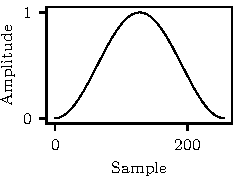
\includegraphics{figure/hann.pdf}
		\caption{A single Hann window.}
		\label{fig.hann}
	\end{subfigure}\quad
	\begin{subfigure}[t]{0.60\textwidth}
		\centering
		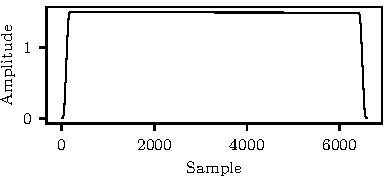
\includegraphics{figure/window_sumsquare.pdf}
		\caption{Sum of 100 overlapping windows. This corresponds to $\mathrm{COLA}_M(n)$ where $0\le n < (100-1) \cdot H + M$.}
		\label{fig.hann-summed}
	\end{subfigure}%
	\caption{Visualization of overlapping Hann windows of size $M=256$ and hop length of $H=64$: $w_M(n)=\frac{1}{2}[1-cos(\frac{2\pi n}{M})]$~\cite{Harris1978}.}
\end{figure}
% Energy loss by window
It is noteworthy that there will be a processing gain by using a window. This means the mean of the power spectrum will be lower by using a window~\cite[p.~83]{Lyons1997}. In order to recover this loss a division by $\sum_{n=0}^{M}w_M(n)$ is needed~\cite[p.~15]{Heinzel2002}.

% Inverse DFT
When separating speech using \gls{dc}, the signal is modified in the frequency-domain. Once the signal has been modified, it is possible to convert it back to time-domain using the \gls{idft}:
\begin{equation}
	x(n) = \frac{1}{N}\sum_{m=0}^{N-1} X(m)e^{-i2\pi m n / N}.
	\label{eq.idft}
\end{equation}
Apart from minor numerical errors the inverse is expected to be the same as the original input.

% FFT
In~\citeyear{Cooley1965}~\textcite{Cooley1965} defined the \gls{fft} which is an efficient implementation of the \gls{dft} to reduce the computational costs for a large amount of samples~\cite[p.~129]{Lyons1997}.~\textcite[p.~131]{Lyons1997} makes clear that the \gls{fft} is not an approximation to the \gls{dft} but in fact is equal. \gls{fft} and \gls{ifft} are going to be used throughout the paper.
Some implementations assume that $N=2^k$, where k is a positive integer~\cite[p.~130]{Lyons1997}, while others are more relaxed.
If the input to the \gls{fft} is real valued, some efficient implementations do not calculate the negative frequencies. Therefore, it is required to scale the linear power spectrum by a factor of two~\cite[p.~15]{Heinzel2002}.

% STFT
In discrete signals like speech the frequencies change over time. A usual approach to make the \gls{dft} dependent on the time is by creating short overlapping windows like demonstrated in Figure \ref{fig.hann-summed}~\cite[p.~714]{Oppenheim1999}.
This \gls{stft} is defined as:
\begin{equation}
	S(t, m) = \sum_{n=0}^{N-1} x(n)w_M^\alpha(n-tH)e^{-i2\pi m n / N}
	\label{eq.stft}
\end{equation}
\cite{Smith2011}.
Here $x(n)$ denotes the real valued discrete signal, $w_M^\alpha$ a window function of length $M$ and $H$ the hop size. The value of $\alpha$ is explained later. Note that for all values of the discrete signal which are outside of the window the product in the sum is zero. In conclusion, the \gls{stft} takes a discrete signal and creates a 2-dimensional function of time and frequency. In practice if $N-M$ is not a multiple of the hop size zero-padding is used to create time intervals of desired size.
% iSTFT
In order to inverse the result of the complex \gls{stft}, Equation \ref{eq.idft} can be used. This yields the equation
\begin{equation}
	x_t(n) = \begin{cases*}
		\frac{1}{M} \sum_{m=0}^{M-1} S(t, m)e^{-i2\pi m (n-tH)) / N}& if $tH \le n < tH + M$ \\
		0      & otherwise
	\end{cases*},
\end{equation}
where $x_t(n):=x(n)w_M^\alpha(n-tH)$ and $\alpha>0$. In order to reconstruct the original signal $x(n)$, overlap-add is required, which is defined by the following sum~\cites[p.~857]{Oppenheim2014}{Sharpe2018}:
\begin{equation}
	\begin{split}
		\sum_{t=-\infty}^{\infty}x_t(n)w_M^\alpha(n-tH)
		&=\sum_{t=-\infty}^{\infty}x(n)w_M^{\alpha+1}(n-tH) \\
		&=x(n)\mathrm{COLA}_M(n)
	\end{split},
\end{equation}
where $\mathrm{COLA}_M(n)=\sum_{t=-\infty}^{\infty}w_M^{\alpha+1}(n-tH)$.
Note that the usage of infinite sums is possible here because $x_t(n)$ is defined on $\mathbb{Z}$.
$\mathrm{COLA}_M$ is visualized in Figure \ref{fig.hann-summed} where the value of $\mathrm{COLA}_M(n)$ is shown for $0\le n < 100 \cdot M$.
Therefore, the reconstructed signal is given by
\begin{equation}
	x(n) = \frac{\sum_{t=-\infty}^{\infty}x_t(n)w_M^\alpha(n-tH)}{\mathrm{COLA}_M(n)}.
\end{equation}
Window functions fulfill the \gls{cola} constraint exactly if and only if $\forall n \in \mathbb{Z}: \mathrm{COLA}_M(n)=C$, where $C$ is some constant.~\cites{Smith2011}[p.~857]{Oppenheim2014}.
If the \gls{stft} $S(t,m)$ is modified arbitrarily to create $\tilde{S}(t,m)$, then there is no discrete signal $\tilde{x}$ which represents the modified \gls{stft}. In order to mitigate this problem \textcite[p.~237 eq. 6]{Griffin1984} reduce the squared error between the modified $\tilde{S}(t,m)$ and the \gls{stft} of $\tilde{x}$ by using $\alpha=1$.

Therefore, it is useful if a window function fulfills \gls{cola} since in this case $x(n)=\frac{x_t(n)}{C}$. If $C=1$ then no division is needed.
Note that it is required that $\forall n \in \mathbb{Z}$: $\mathrm{COLA}_M(n)$ isn't zero.
A periodic (\gls{dft}-even) Hann window fulfills \gls{cola} with a window size of $M+1$ and hop size of $0.25M$~\cite[p.~859]{Oppenheim2014}.
The inverse \gls{stft} approach used in \gls{dc} is the overlap-add method with $\alpha=1$ and a three-quarter overlapping Hann window.

A close look at Figure \ref{fig.hann-summed} reveals that for samples at the beginning or near the end $\mathrm{COLA}_M(n)$ is almost zero. Therefore, parts of the signal are basically lost. In this thesis samples of value zero are added to the start and end of signal $x$ such that the first Hann window is at centered at $tH$. After reconstructing the signal, some samples have to be truncated.

One might ask why the rectangular window which obviously fulfills the \gls{cola} criterion is not a good choice. The reason is the already discussed leakage effect.

In this section the \gls{dft} and \gls{fft} were introduced and basic constrains covered. Based on this the \gls{stft} was introduced which is the main algorithm which will be used to create features and reconstruct discrete signals. Also, the main ideas behind choosing a window were covered.

In the thesis' implementation of \gls{dc} the \gls{fft} implementation of the \texttt{NumPy} library is used~\cite{Oliphant2006}. The implementation of the \gls{stft} which uses the \gls{fft} from NumPy is found in the \texttt{librosa} library~\cite{McFee2019}.

\section{Deep Neural Networks}\label{sec.foundations-dnn}
% No free lunch theorem p. 113
% Universal Approximation Properties and Depth

The basic instance of neural networks is the feedforward neural network. It is also called \glspl{mlp} and is a typical and basic model in modern machine learning. The goal of a \gls{mlp} is to estimate some function $f^{*}$ by learning from samples. For each sample $x$ the function $f^{*}$ gives a result $\hat{y}=f^{*}(x)$. The neural network tries to estimate $f^{*}$ by using the model $y=f(x;\theta)$ such that $y \approx \hat{y}$, where $\theta$ are the learned weights. The notation $f(x;\theta)$ means that $f$ is a function of $x$ and is parameterized by $\theta$. This notation is used throughout this section.
By learning the function $f^{*}$ the weights $\theta$ are adjusted incrementally. The goal is that the network does not only optimize the weights such that already seen inputs are mapped correctly, but that $f$ also works for unseen inputs. This is also known as generalization.
Usually a training set is used to optimize the weights and a testing or evaluation set is used to measure the performance. \cite[p.~102]{Goodfellow2016}

We go shortly about the terminology which is used with neural networks. Multiple functions get chained together in order to build the model. For example the three functions $f_1$, $f_2$ and $f_3$ can represent a neural network if they are composed to one function $f(x)=(f_1 \circ f_2 \circ f_3)(x)=f_1(f_2(f_3(x)))$. Each of these functions represents one layer. Therefore, this network has a depth of three, where the third layers is called the output layer, the first input layer and the layer in between hidden layer.
The number of the variables of each layer determines the width of it.
The term ''neural'' is derived from neuroscience after observing patterns which reveal the representation ability of the brain. If a vector is passed to a layer, each variable in the layer is treated like a neuron, which can decide on its own what the output value should be. In the case of an artificial neural network the output value is determined by the weight and bias of the neuron. In practice, however, this can be seen as an analogy and only inspires the engineering of neural networks.~\cite[p.~163]{Goodfellow2016}

An intuitive way to introduce feedforward neural networks is to start with a linear model which is not able to properly approximate a nonlinear function like for example, $x^2$. In case of linear regression the model is $y=w\tran x+b$~\cite[p.~106]{Goodfellow2016}. This model can be extended to use $\phi(x)$ instead of $x$ directly, where $\phi$ denotes a nonlinear hidden layer. This yields the nonlinear model $y=w\tran \phi(x)+b$. One might question how $\phi$ should be constructed. The answer is that we actually leave this task to the neural network.
Therefore, the model of the complete \gls{mlp} is defined as $f(x;\theta,b,w)=\phi(x;\theta,b)\tran w$, where $\theta$ are the weights of a hidden layer and $w$ the weights which map from the hidden layer to the output layer.
At this point, engineers can also apply their domain knowledge to restrict the function family $\phi$ for each hidden layer. Nevertheless, this task is usually left completely to the neural network.~\cite[p.~165]{Goodfellow2016}

% Activation functions
The function of a nonlinear hidden layer $\phi$ is defined as $\phi(x;\theta,b)=g(\theta\tran x+b)$~\cite[p.~167]{Goodfellow2016}. This function involves a nonlinear activation function $g$.
The qualification of activation functions and its utilization cases will be discussed in Section \ref{sec.mlp-activations}.

In Figure \ref{fig.mlp-visualization} a simple feedforward neural network is presented. In each hidden layer a specific activation function $g \in \{g_1,g_2\}$, weight matrix $\theta \in \{\theta_1,\theta_2\}$ and bias vector $b \in \{b_1,b_2\}$ is used. The computation in the output layer is indicated by a so far undefined function  $\hat{f}_{w,b_3}$ which will be discussed in Section \ref{sec.mlp-activations}. Taking $x$ as input the whole neural network outputs $y$, depending on the network architecture. Evaluating $y$ is also called forward propagation, which is achieved by recursively computing the activations in each layer until the last one is reached.
\begin{figure}
	\centering
	\begin{tikzpicture}[shorten >=1pt,->, node distance=1.8cm]
		\tikzstyle{every pin edge}=[<-,shorten <=1pt]
		\tikzstyle{annot} = [text width=4em, text centered]

		\node[output neuron] (O) at (0,0) {$y$};
		\node[hidden neuron, below of=O] (H-3) {$a_2$};
		\node[hidden neuron, below of=H-3] (H-2) {$a_1$};
		\node[input neuron, below of=H-2] (I-1) {$x$};

		\path (I-1) edge node[right]{$a_1=g_1(\theta_1\tran x+b_1)$} (H-2);
		\path (H-2) edge node[right]{$a_2=g_2(\theta_2\tran a_1+b_2)$} (H-3);
		\path (H-3) edge node[right]{$y=\hat{f}_{w,b_3}(a_2)$} (O);
	\end{tikzpicture}
	\caption{Architecture of a simple \gls{mlp} with the computational steps needed in order to calculate the activations $a_1$, $a_2$ and $y$ given the input $y$. In this example the weights are given by $\theta_1,\theta_2$, the biases by $b_1,b_2$ and the activation functions by $g_1,g_2$. The function $\hat{f_w}$ is not yet defined as it needs to be chosen carefully according the task of the perceptron.}
	\label{fig.mlp-visualization}
\end{figure}
The process of training a model involves the optimization using back-propagation of the weights which will be discussed in Chapter \ref{sec.mlp-backpropagation}~\cite[p.~165]{Goodfellow2016}. \textcite{Goodfellow2016} point out that the term back-propagation is often misunderstood. The back-propagation algorithm only computes the gradients whereas algorithms like gradient descent are responsible for updating the weights and biases.

\subsection{Loss and Activation Functions}\label{sec.mlp-cost-function}\label{sec.mlp-activations}

Machine learning algorithms require a loss function as feedback to evaluate how good an estimation is. As noted in the introduction, the goal is to approximate the function $f$ to $f^*$.
A loss function rates how well the model performs based on its current weights and biases. Minimizing the loss function and finding good weights and biases is an optimization problem.
The difference between an optimization problem and machine learning is that the latter tries to generalize the estimated function such that it also works good on previously unseen testing data.
Because the model of neural networks is nonlinear, the loss function is inherently nonlinear.
This causes the loss function to be convex and therefore there is no guarantee that gradient descent will find a global minimum~\cite[p.~171]{Goodfellow2016}.
One might ask how the weights and biases should be initialized. According to~\textcite[p.~172]{Goodfellow2016} weights should be initialized to small random values and the biases to zero or small positive random values.

There are multiple loss functions to choose from, namely cross-entropy, \gls{mse} and \gls{mae}. \textcite[p.~175]{Goodfellow2016} notice that depending on the transformations in the output layer, the loss functions \gls{mse} and \gls{mae} can perform poorly. The commonly used cross-entropy loss is based on the maximum likelihood estimation and performs well in a lot of applications.

Depending on the task of the network the output layer has to be selected carefully because of the effect of saturation. Therefore, this chapter will find out in which way the function $\hat{f}_{w,b_3}$ in Figure \ref{fig.mlp-visualization} has to be chosen in order to complete the computation of $y$.

A function saturates if the function becomes very flat for specific input parameters. For example the derivative of the logistic function $\sigma(x)=\frac{1}{1+e^{-x}}$ is very small for positive and negative values. If a function saturates for specific values numerical errors will arise which make gradient-based algorithms perform poorly.~\cite[p.~173]{Goodfellow2016}

The first possibility is that the output layer is linear. In this case $y=\hat{f}_{w,b_3}(a_2)=w\tran a_2+b_3$, which does not saturate.~\cite[p.~176]{Goodfellow2016}

If the task of the network is to perform binary classification to separate for example cats and dogs, then the logistic curve is a proper choice for the activation function when combining it with maximum likelihood. This yields the following output layer: $y=\sigma(w\tran a_2+b_3)$.~\cite[p.~176-178]{Goodfellow2016}

Lastly, if the task of the network is to predict $n$ different classes a softmax output layer should be considered the right choice. Due to the insignificance for the \gls{dc} approach this will not be discussed in further detail.~\cite[p.~179]{Goodfellow2016}

The \gls{dc} approach uses a fully connected layer as output layer. Therefore we don't have to deal with the effect of saturation when choosing the loss function in Section \ref{sec.loss-dc}.

After choosing an activation function for the output layer, further functions have to be evaluated for the hidden layers.
The selection of an activation function for each hidden layer is still a process of trial and error and an active research field. The usual method is to compare the efficiency of the network using different activation functions.
It was already mentioned that in order to train a neural network it is necessary to determine the derivatives of the loss function and therefore also the derivatives of the activation functions. One could think that it in the context of neural networks it is required that these functions are differentiable. Nevertheless, the common rectifier activation function
\begin{equation}
	g_{ReL}(x)=\max(0, x)
	\label{eq.re}
\end{equation}
is not differentiable at $x_0=0$ because $\lim_{x \rightarrow 0} \frac{g_{ReL}(x)-g_{ReL}(x_0)}{x-x_0}=0$ for $x<0$ and for $x>0$ it is 1.
\textcite[p.~186]{Goodfellow2016} explain that in practice this is not required because gradients usually do not approach $x_0=0$ and therefore cases where the derivative is undefined are uncommon. Also when implementing these networks in software it is very likely that if the gradient is computed to be 0 that it actually is not really 0.

The linear rectifier unit as seen in \ref{fig.mlp-activation-functions.relu} and defined in Equation \ref{eq.re} is a common activation function. The nature of this function makes the layer for the most part linear. Only negative values are clipped to 0. This linearity makes the model easier to optimize~\cite[p.~188]{Goodfellow2016}.
As already mentioned in Section \ref{sec.mlp-cost-function}, it makes sense to initialize the biases to a small positive value such that neurons are active in the initial state.
\textcite[p.~189]{Goodfellow2016} note that especially \glspl{rnn} benefit from this activation function because of its linearity.
The leaky linear rectifier unit as seen in Figure \ref{fig.mlp-activation-functions.leaky-relu}
\begin{equation}
	g_{LReL}(x)=\begin{cases*}
		x 			& if $x > 0$ \\
		0.01x      & otherwise
	\end{cases*}
\end{equation}
represents a variation, which has a small slope if $x<0$ with the result that there is always a non-zero small gradient~\cite{Maas2013}.

Other activation functions are the logistic function and the hyperbolic tangent function. It was already mentioned that the logistic curve saturates for very positive and negative values (see Figure \ref{fig.mlp-activation-functions.sigmoid}). The same holds true for the hyperbolic tangent function as seen in Figure \ref{fig.mlp-activation-functions.tanh}.
Therefore, the use of these is functions in \glspl{mlp} is uncommon today.
Nevertheless, the hyperbolic tangent activation function performs well in the \gls{dc} approach.
It is noteworthy that the tangent is more similar to a linear mapping compared to the logistic function because for the interval $[0,1]$ the tangent is more similar to a linear function.~\cite[p.~189]{Goodfellow2016}

\begin{figure}
	\centering
	\begin{subfigure}[t]{0.25\textwidth}
		\centering
		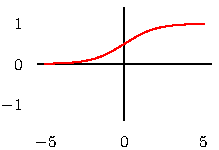
\includegraphics{figure/sigmoid.pdf}
		\caption{Logistic Sigmoid}
		\label{fig.mlp-activation-functions.sigmoid}
	\end{subfigure}%
	\begin{subfigure}[t]{0.25\textwidth}
		\centering
		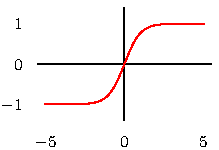
\includegraphics{figure/tanh.pdf}
		\caption{Hyperbolic Tangent}
		\label{fig.mlp-activation-functions.tanh}
	\end{subfigure}%
	\begin{subfigure}[t]{0.25\textwidth}
		\centering
		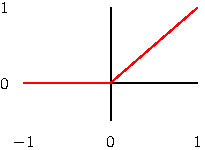
\includegraphics{figure/relu.pdf}
		\caption{Linear Rectifier Unit}
		\label{fig.mlp-activation-functions.relu}
	\end{subfigure}%
	\begin{subfigure}[t]{0.25\textwidth}
		\centering
		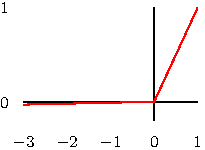
\includegraphics{figure/leaky_relu.pdf}
		\caption{Leaky Rectifier Unit}
		\label{fig.mlp-activation-functions.leaky-relu}
	\end{subfigure}%
	\caption{Overview of the common activation functions used in \glspl{mlp}.}
	\label{fig.mlp-activation-functions}
\end{figure}


\subsection{Back-propagation and Gradient Descent}\label{sec.mlp-backpropagation}
% TODO: Make first layer l=0 instead of l=1

If we want to calculate $y=f(x)$ using a trained feedforward neural network we iterate the network in forward direction. In the case of an untrained \gls{mlp} the output is more or less random. Therefore, some kind of feedback is required to update the weights and biases in order to train it. In Chapter \ref{sec.mlp-cost-function} the loss function was introduced which gives a metric on how well the network performs. The goal of this chapter is to give an intuition how the derivative of the loss function $J$ in respect to the weights of each layer is determined.
$J(W, B)$ gives the loss between the estimated $y$ and the expected $\hat{y}$, where $W=(\theta_1, \theta_2, \ldots, \theta_L)$ contains the weights and $B=(b_1, b_2, \ldots, b_L)$ the biases for layer 1 to $L$.
This allows algorithms like gradient descent to update the weights according to the derivatives. The adjustment for each weight depends on the derivative in respect to the current weights. \cite[p.~198]{Goodfellow2016}

This chapter is structured in three parts. In the first one the back-propagation algorithm is presented for a simplified \gls{mlp}. The second part notes that the algorithm can generalized for arbitrary \glspl{mlp}. Last the idea behind gradient descent is explained.

A simple model which can demonstrate back-propagation is a \gls{mlp} where each layer has only a single neuron. Note that in this case each layer has only a single weight and a single bias. Therefore, no multiplication of multi-element vectors is needed in the simple model. In order to visualize this, a computational graph is presented in Figure \ref{fig.mlp-single-neuron}. The training of the network works by adjusting the weights and biases. Therefore, we want to calculate $\frac{dJ}{d\theta_l}$ and $\frac{dJ}{db_l}$ for each layer. A closer look at the computational graph reveals that the activation $a_{L}$ of the last layer $L$ depend on $z_{L}$ and therefore also on the weight, bias and activation of the previous layer. \cite[p.~201]{Goodfellow2016}
\begin{figure}
	\centering
	\begin{tikzpicture}[sibling distance=2cm, level distance=1cm,
			every node/.style = {shape=rectangle, rounded corners,align=center}]]
		\node {$J$} [grow=up]
		child { node {$\hat{y}$} }
		child { node {$a_{L}$}
				child { node {$z_{L}$}
						child { node {$\theta_{L}$} }
						child { node {$a_{L-1}$} child { node {$z_{L-1}$}
										child { node {$\theta_{L-1}$} }
										child { node {$a_{L-2}$} child { node {...}}}
										child { node {$b_{L-1}$} }
									}}
						child { node {$b_{L}$} }
					}
			};
	\end{tikzpicture}
	\caption{The computational graph of a multilayer neural network where each layer has exactly one neuron. $L$ denotes the layer layer in the network. Therefore, $\theta_L$ is the weight, $b_L$ the bias and $a_L=g(z_L)$ the activation of the last layer. $J$ is the loss function which compares the activation with the expected results $\hat{y}$.}
	\label{fig.mlp-single-neuron}
\end{figure}

The core of the back-propagation algorithm is the chain rule which allows to calculate the derivative of a function $f = g \circ h$ if the derivatives of $g$ and $h$ are already known.
Using this rule it is possible to determine the derivative of the loss in respect to the weight $\theta_{L}$ of the last layer $L$ using the following equation:
\begin{equation}
	\frac{\partial J}{\partial \theta_{L}}
	=
	\frac{\partial z_{L}}{\partial \theta_{L}}
	\frac{\partial a_{L}}{\partial z_{L}}
	\frac{\partial J}{\partial a_{L}}.
	\label{eq.mlp-simple-weight-derivative}
\end{equation}
Let's recall that the formula of the hidden layer $l$ is
\begin{equation}
	a_l = g_l(z_l),
	\label{eq.mlp-forward-propagation}
\end{equation}
where
\begin{equation}
	z_l=\theta_l\tran  a_{l-1} + b_l
\end{equation}
like shown in Figure \ref{fig.mlp-visualization}.
The term in the middle on the right side of Equation \ref{eq.mlp-simple-weight-derivative} is the derivative of the activation in respect to $z_{L}$, which is $g_{L}'(z_{L})$.
The first term on the right is equal to the activation of the previous layer $a_{L-1}$. This is because $z_{L}$ is defined as $z_{L}=\theta_l\tran a_{L-1} + b_{L}$ and therefore $a_{L-1}$ is the slope.

In summary, Equation \ref{eq.mlp-simple-weight-derivative} can also be expressed as
\begin{equation}
	\frac{\partial J}{\partial \theta_{L}}
	= a_{L-1} \delta_{L},
\end{equation}
where $\delta_{L}=\frac{\partial J}{\partial a_{L}}g_{L}'(z_{L})$. Similarly if the derivative of the loss function in respect to the bias is
\begin{equation}
	\frac{\partial J}{\partial b_{L}}
	= \delta_{L}
\end{equation}
(The factor $a_{L-1}$ is omitted here because $\frac{\partial z_{L}}{\partial b_{L}}=1$).

After calculating the derivatives for the last layer we can calculate the derivatives for the hidden layers. Using the chain rule it is possible to calculate the derivative in respect to the activations of the previous layer:
\begin{equation}
	\frac{\partial J}{\partial a_{L-1}}
	= \frac{\partial z_{L}}{\partial a_{L-1}}
	\frac{\partial a_{L}}{\partial z_{L}}
	\frac{\partial J}{\partial a_{L}}
	= \theta_L\tran  \delta_L.
\end{equation}

This equation can be used when calculating the derivative of $J$ with respects to the weight of the layer $L-1$:
\begin{equation}
	\begin{split}
		\frac{\partial J}{\partial \theta_{L-1}}
		& = \frac{\partial z_{L-1}}{\partial \theta_{L-1}}
		\frac{\partial a_{L-1}}{\partial z_{L-1}}
		\frac{\partial z_{L}}{\partial a_{L-1}}
		\frac{\partial a_{L}}{\partial z_{L}}
		\frac{\partial J}{\partial a_{L}} \\
		& = \frac{\partial z_{L-1}}{\partial \theta_{L-1}}
		\frac{\partial a_{L-1}}{\partial z_{L-1}}
		\frac{\partial J}{\partial a_{L-1}} \\
		& = a_{L-2} \, \theta_L\tran  \delta_L \, g_{L-1}'(z_{L-1}).
	\end{split}
\end{equation}

Using the chain rule we can recursively determine all the derivatives in the computational graph by repeating the above computation from $l=L$ until $L=1$.
This is the main idea of back-propagation. Although the algorithm was only demonstrated for scalar values it also applies to vectors and tensors of arbitrary dimension~\cite[p.~199]{Goodfellow2016}. If dealing with vectors the chain rule can be expressed as
\begin{equation}
	\triangledown(x,z)=(\frac{\partial y}{\partial x})\tran  \triangledown(y,z),
\end{equation}
where $x \in \mathbb{R}^m, y \in \mathbb{R}^n, g: \mathbb{R}^m \rightarrow \mathbb{R}^n, f: \mathbb{R}^n \rightarrow \mathbb{R}$, $\frac{\partial y}{\partial x}$ the $n \times m$ Jacobian matrix and $z=f(y)$ with $y=g(x)$~\cite[p.~199]{Goodfellow2016}. This allows the weight vectors to have an arbitrary dimension in a generalized version of gradient-descent.

After calculating the derivatives it is possible to update the weights and biases of each layer $l$ using gradient descent
\begin{equation}
	\theta_l \leftarrow \theta_l - \eta \frac{\partial J}{\theta_l}
\end{equation}
and biases
\begin{equation}
	b_l \leftarrow b_l - \eta \frac{\partial J}{b_l},
\end{equation}
where $\eta$ is the learning rate~\cite[Chapter~2]{Nielsen2015}.
Even though it is possible to update the weights after each input it can also be done in batches. This means the weight adjustments are collected over $b_s$ inputs before the model is actually updated. \cite[p.~272]{Goodfellow2016}

In this section we covered how the back-propagation works. Armed with that knowledge we can discuss how \glspl{rnn} work in the next section.

\subsection{Recurrent Neural Networks} \label{sec.rnn}

The network architecture of \gls{dc} is based on \glspl{rnn}. To be more accurate a bidirectional \gls{lstm} architecture was chosen in~\cite{Hershey2016} which will be covered later in this section.
The difference between feedforward and recurrent neural networks is that the latter allows recurrent connections between hidden neurons whereas the former doesn't. The reason for this architectural decision is that it is quite difficult for a \gls{mlp} to model time-series data. The connections between neurons within a layer allows interactions between present and future inputs.~\cite[p.~22]{Graves2012}.

Especially for audio signals containing speech, temporal context is important.
If a recurrent network is fed with audio data it is beneficial if the output of the time step $t+1$ depends on the activations of the time step $t$.

The recurrent network expects a sequence of features as input. Therefore, the input is not only a vector of features, but a matrix $I=\begin{psmallmatrix}x^{(1)} & x^{(2)} & \ldots & x^{(t)}\end{psmallmatrix}\tran $ where each row corresponds to a feature vector. Note the superscript in brackets is not an exponent but just another index. For each time step $t=1$ until $t=\tau$ the vector $x^{(i)}$ is fed into the \gls{rnn}. % Notation of vectors in matrix

In Figure \ref{fig.rnn} a visualization of a \gls{rnn} can be viewed where the connections between the hidden layers represent the time-dependence between samples in the sequence of inputs. The shape of the input in each time step is still the same as in the \gls{mlp} shown in Figure \ref{fig.mlp-visualization}.

\begin{figure}
	\centering
	\begin{tikzpicture}[node distance=0.5cm]
    % Hidden cells
    % Empty rectangle
    \node[rectangle] (Y0) at (0, 0) {};
    \node[cell neuron, right=2em of Y0] (RNN) {\sigmoidfigure};
    \node[cell neuron, right=of RNN] (RNN2) {\sigmoidfigure};
    \node[cell neuron, right=of RNN2] (RNN3) {\sigmoidfigure};
    \node[cell neuron, right= of RNN3] (RNN4) {\sigmoidfigure};
    % Empty rectangle
    \node[rectangle, right=2em of RNN4] (RNN5) {};

    % Input/Output neurons
    \node[input neuron, below=of RNN] (X1) {$x^{(t-2)}$};
    \node[input neuron, below=of RNN2] (X2) {$x^{(t-1)}$};
    \node[input neuron, below=of RNN3] (X3) {$x^{(t)}$};
    \node[input neuron, below=of RNN4] (X4) {$x^{(t+1)}$};
    \node[output neuron, above=of RNN4] (Y5) {$y^{(t+1)}$};
    \node[output neuron, above=of RNN3] (Y4) {$y^{(t)}$};
    \node[output neuron, above=of RNN2] (Y3) {$y^{(t-1)}$};
    \node[output neuron, above=of RNN] (Y2) {$y^{(t-2)}$};

    \node[rectangle, left=of RNN, text width=2.5cm] {Hidden Layer};
    \node[rectangle, left=of X1, text width=2.5cm] {Input Layer};
    \node[rectangle, left=of Y2, text width=2.5cm] {Output Layer};

    \draw[-stealth, thick] (X1) -- (RNN);
    \draw[-stealth, thick] (X2) -- (RNN2);
    \draw[-stealth, thick] (X3) -- (RNN3);
    \draw[-stealth, thick] (X4) -- (RNN4);

    \draw[-stealth, thick] (RNN) -- (Y2);
    \draw[-stealth, thick] (RNN2) -- (Y3);
    \draw[-stealth, thick] (RNN3) -- (Y4);
    \draw[-stealth, thick] (RNN4) -- (Y5);


    % Arrow labels between hidden cells
    \draw[-stealth, thick] (RNN) -- (RNN2);
    \draw[-stealth, thick] (RNN2) -- (RNN3);
    \draw[-stealth, thick] (RNN3) -- (RNN4);

    %  Dotted arrows
    \draw[-stealth, thick, densely dotted] (Y0) -- (RNN);
    \draw[-stealth, densely dotted, thick] (RNN4) -- (RNN5);
\end{tikzpicture}
	\caption{Unfolded architecture of a simple \gls{rnn} over time. Each column is similar to the \gls{mlp} structure of Figure \ref{fig.mlp-visualization} and represents a single time step. This figure shows an extract of a \gls{rnn} for the time steps $t-2$ until $t+1$. Each hidden layer depends on the hidden layer one time step earlier.}
	\label{fig.rnn}
\end{figure}

The forward-propagation equation for each layer $l$ is
\begin{equation}
	a^{(t)}_l=g_l(z^{(t)}_l)
	\label{eq.rnn-forward}
\end{equation}
with
\begin{equation}
	z^{(t)}_l=U a^{(t)}_{l-1} + W a^{(t-1)}_l + b_l,
\end{equation}
where $g_l$ is an activation function, $b_l$ the biases, $\theta_l$ input-to-hidden weights, $w_l$ hidden-to-hidden weights, $a^{(t)}_{l-1}$ the activations of the previous layer and $a^{(t-1)}_l$ the activations of the previous time step of the same layer~\cite[p.~370]{Goodfellow2016}.
Note that for each time step the initial input $a^{(t)}_0$ of the network is $x_{(t)}$.
The Equation \ref{eq.rnn-forward} is quite similar to Equation \ref{eq.mlp-forward-propagation}. The difference is that the activation of each layer depends not only on the previous layer but also on the activations in the past.

The forward-propagation algorithm starts with $t=1$ and recursively determines the activations until $t=\tau$. For simplicity he initial value of $a^{(0)}_l$ is considered to be zero~\cite[p.~23]{Graves2012}.
The output of the last layer the can be computed using a fully connected layer which follows Equation \ref{eq.mlp-forward-propagation}.

A possible back-propagation algorithms for \glspl{rnn} is \gls{bptt}. This algorithm works similar to the procedure described in Section \ref{sec.mlp-backpropagation}. It applies the back-propagation algorithm for \glspl{mlp} at each time step from $t=\tau$ to $t=0$ and determines the updates for the weights in each step.~\cite[p.~450]{Williams1995}
Similar to the \glspl{mlp} the weight updates can happen here also in batches of size $b_s$.

\subsubsection{Long Short-term Memory}\label{sec.lstm}

A common problem when dealing with \glspl{rnn} is the vanishing gradient problem. The use of \gls{lstm} cells together with recurrent networks aims to solve this problem.

The vanishing gradient problem prevents the formation of long-term dependencies between samples in a sequence~\cite[p.~38]{Graves2012}. 
This is because there is no memory and control mechanism which defines how volatile the calculated results are. 
This effect is best demonstrated using a graphic which can be seen in \ref{fig.vanishing-gradient}.
\begin{figure}[b]
	\centering
	\begin{tikzpicture}[node distance=0.5cm]
    % Hidden cells
    % Empty rectangle
    \node[rectangle] (Y0) at (0, 0) {};
    \node[cell neuron, fill=black, right=2em of Y0] (RNN) {};
    \node[cell neuron, fill=black!50, right=of RNN] (RNN2) {};
    \node[cell neuron, fill=black!25, right=of RNN2] (RNN3) {};
    \node[cell neuron, fill=black!12, right= of RNN3] (RNN4) {};
    % Empty rectangle
    \node[rectangle, right=2em of RNN4] (RNN5) {};

    % Input/Output neurons
    \node[input neuron,fill=black, text=white, below=of RNN] (X1) {$x^{(t-2)}$};
    \node[input neuron, below=of RNN2] (X2) {$x^{(t-1)}$};
    \node[input neuron, below=of RNN3] (X3) {$x^{(t)}$};
    \node[input neuron, below=of RNN4] (X4) {$x^{(t+1)}$};
    \node[output neuron, fill=black!12, above=of RNN4] (Y5) {};
    \node[output neuron, fill=black!25, above=of RNN3] (Y4) {};
    \node[output neuron, fill=black!50, above=of RNN2] (Y3) {};
    \node[output neuron, fill=black, above=of RNN] (Y2) {};

    \node[rectangle, left=of RNN, text width=2.5cm] {Hidden Layer};
    \node[rectangle, left=of X1, text width=2.5cm] {Input Layer};
    \node[rectangle, left=of Y2, text width=2.5cm] {Output Layer};

    \draw[-stealth, thick] (X1) -- (RNN);
    \draw[-stealth, thick] (X2) -- (RNN2);
    \draw[-stealth, thick] (X3) -- (RNN3);
    \draw[-stealth, thick] (X4) -- (RNN4);

    \draw[-stealth, thick] (RNN) -- (Y2);
    \draw[-stealth, thick] (RNN2) -- (Y3);
    \draw[-stealth, thick] (RNN3) -- (Y4);
    \draw[-stealth, thick] (RNN4) -- (Y5);


    % Arrow labels between hidden cells
    \draw[-stealth, thick] (RNN) -- (RNN2);
    \draw[-stealth, thick] (RNN2) -- (RNN3);
    \draw[-stealth, thick] (RNN3) -- (RNN4);

    %  Dotted arrows
    \draw[-stealth, thick, densely dotted] (Y0) -- (RNN);
    \draw[-stealth, densely dotted, thick] (RNN4) -- (RNN5);
\end{tikzpicture}
	\caption{Visualization of a the vanishing gradient effect. The monochromic gradient of each layer represents the sensitivity to the inputs $x^{(t-2)}$ to $x^{(t+1)}$. The influence from the inputs vanishes slowly over time. This figure is redrawn from~\cite[p.~38]{Graves2012}.}
	\label{fig.vanishing-gradient}
\end{figure}
As time progresses the influence of the input slowly decays. In the following paragraphs a cell structure is presented which counteracts this effect. The suggested cell structure controls how influential the activations of the input and hidden layers are. Furthermore, a mechanism of forgetting is required.

\begin{figure}
	\centering
	\begin{tikzpicture}[
    % GLOBAL CFG
    font=\scriptsize,
    >=LaTeX,
    % Styles
    cell/.style={% For the main box
        rectangle, 
        rounded corners=5mm, 
        draw,
        very thick,
        },
    operator/.style={%For operators like +  and  x
        circle,
        draw,
        inner sep=-0.5pt,
        minimum height =.2cm,
        },
    function/.style={%For functions
        ellipse,
        draw,
        inner sep=1pt
        },
    ct/.style={% For external inputs and outputs
        circle,
        draw,
        line width = .75pt,
        minimum width=1cm,
        inner sep=1pt,
        },
    gt/.style={% For internal inputs
        rectangle,
        draw,
        minimum width=4mm,
        minimum height=3mm,
        inner sep=0pt
        },
    mylabel/.style={% something new that I have learned
        font=\scriptsize
        },
    ArrowC1/.style={% Arrows with rounded corners
        rounded corners=.25cm,
        thick,
        },
    ArrowC2/.style={% Arrows with big rounded corners
        rounded corners=.5cm,
        thick,
        },
    ]

%Start drawing the thing...    
    % Draw the cell: 
    \node [cell, minimum height =4cm, minimum width=6cm] at (0,0){} ;

    % Draw inputs named ibox#
    \node [gt] (ibox1) at (-2,-0.75) {\sigmoidfigure};
    \node [gt] (ibox2) at (-1.5,-0.75) {\sigmoidfigure};
    \node [gt, minimum width=1cm] (ibox3) at (-0.5,-0.75) {$\tanh$};
    \node [gt] (ibox4) at (0.5,-0.75) {\sigmoidfigure};

   % Draw opérators   named mux# , add# and func#
    \node [operator] (mux1) at (-2,1.5) {$\times$};
    \node [operator] (add1) at (-0.5,1.5) {+};
    \node [operator] (mux2) at (-0.5,0) {$\times$};
    \node [operator] (mux3) at (1.5,0) {$\times$};
    \node [function] (func1) at (1.5,0.75) {$\tanh$};

    % Draw External inputs? named as basis c,h,x
    \node[ct] (c) at (-4,1.5) {$C^{(t-1)}$};
    \node[ct] (h) at (-4,-1.5) {$a^{(t-1)}$};
    \node[ct] (x) at (-2.5,-3) {$x^{(t)}$};

    % Draw External outputs? named as basis c2,h2,x2
    \node[ct, label={[mylabel]Cell State}] (c2) at (4,1.5) {$C^{(t)}$};
    \node[ct, label={[mylabel]Activations}] (h2) at (4,-1.5) {$a^{(t)}$};
    \node[ct, label={[mylabel]left:Output}] (x2) at (2.5,3) {$a^{(t)}$};

% Start connecting all.
    %Intersections and displacements are used. 
    % Drawing arrows    
    \draw [->, ArrowC1] (c) -- (mux1) -- (add1) -- (c2);

    % Inputs
    \draw [ArrowC2, color=gray] (h) -| (ibox4);
    \draw [ArrowC1] (h -| ibox1)++(-0.5,0) -| (ibox1); 
    \draw [ArrowC1, color=blue] (h -| ibox2)++(-0.5,0) -| (ibox2);
    \draw [ArrowC1] (h -| ibox3)++(-0.5,0) -| (ibox3);
    \draw [ArrowC1, color=blue] (x) -- (x |- h)-| (ibox3);

    \draw [ArrowC1, color=red] (h) -- (x |- h)-| (ibox1);
    \draw [ArrowC1, color=red] (x) -- (x |- h)-| (ibox1);

    % Internal
    \draw [->, ArrowC2, color=red] (ibox1) -- node[left] {$f^{(t)}$} (mux1);
    \draw [->, ArrowC2, color=blue] (ibox2) |- node[above] {$i^{(t)}$} (mux2);
    \draw [->, ArrowC2, color=blue] (ibox3) -- node[left] {$\tilde{C}^{(t)}$} (mux2);
    \draw [->, ArrowC2, color=gray] (ibox4) |- node[left] {$o^{(t)}$} (mux3);
    \draw [->, ArrowC2] (mux2) -- (add1);
    \draw [->, ArrowC1, color=gray] (add1 -| func1)++(-0.5,0) -| (func1);
    \draw [->, ArrowC2, color=gray] (func1) -- (mux3);

    %Outputs
    \draw [->, ArrowC2] (mux3) |- (h2);
    \draw (c2 -| x2) ++(0,-0.1) coordinate (i1);
    \draw [-, ArrowC2] (h2 -| x2)++(-0.5,0) -| (i1);
    \draw [->, ArrowC2] (i1)++(0,0.2) -- (x2);

\end{tikzpicture}
	\caption{Visualization of a \gls{lstm} cell, where $f$ is the forget gate, $i$ is the input gate and  $o$ is the output gate.}
	\label{fig.lstm-cell}
\end{figure}

First we discuss how a cell ''forgets''. This is visualized by the red part in Figure \ref{fig.lstm-cell}. The input and the activations from the previous time step are combined to get values between 0 and 1 which will later be multiplied by the previous cell state $C^{(t-1)}$:
\begin{equation}
	f^{(t)}=\sigma\Big(U^f x^{(t)} + W^f a^{(t-1)} + b^f\Big),
\end{equation}
where $\sigma$ is the logistic function, $x^{(t)}$ is the input vector, $a^{(t-1)}$ the activations from the previous layer and $U^f$,$W^f$ and $b^f$ the weights and biases of the forget gate. Note that these calculations can be seen as layers within a cell.~\cite[p.~399]{Goodfellow2016}

Secondly the \gls{lstm} needs a way to determine which new information from the input should be added to the cell state. This part is colored blue in Figure \ref{fig.lstm-cell}.
A logistic and hyperbolic tangent layer are responsible for calculating the state update.
The logistic layer determines which values should be updated:
\begin{equation}
	i^{(t)}=\sigma\Big(U^i x^{(t)} + W^i a^{(t-1)} + b^i\Big).
\end{equation}
The tangent layer calculates the values to be added:
\begin{equation}
	\tilde{C}^{(t)}=\tanh\Big(U^C x^{(t)} + W^C a^{(t-1)} + b^C\Big).
\end{equation}
The new state can be calculated using the previous two results:
\begin{equation}
	C^{(t)}=f^t \odot C^{(t-1)} + i^{(t)} \odot \tilde{C}^{(t)},
\end{equation}
where $\odot$ is the element-wise product.
The new state depends on the previous state $C^{(t-1)}$ multiplied by the forget gate $f^{(t)}$ and the modified inputs $\tilde{C}^{(t)}$ multiplied by the input gate $i^{(t)}$. Note that the gates basically act like a filter here. Therefore, the cell is able to remember and also forget.~\cite[p.~399]{Goodfellow2016}

Finally, the output of the cell needs to be calculated. The output gate is implemented as a logistic layer which is filtered using the hyperbolic tangent of the current state:
\begin{equation}
	o^{(t)}=\sigma\Big(U^o x^{(t)} + W^o a^{(t-1)} + b^o\Big),
\end{equation}
\begin{equation}
	a^{(t)}=o^{(t)} \odot \tanh(C^{(t)}).
\end{equation}
The resulting activations $a^{(t)}$ are the activations of the \gls{lstm} cell at time step $t$.~\cite[p.~399]{Goodfellow2016}

Like \glspl{rnn}, \gls{lstm} networks can use the \gls{bptt} algorithm for back-propagation of the loss~\cite[p.~43]{Graves2012}. A difference is that the computation of the derivatives consumes more computing resources are more terms are involved.

\subsubsection{Bidirectional Recurrent Neural Networks}\label{sec.bidi-rnn}

Vanilla \glspl{rnn} and vanilla \gls{lstm} networks are limited in a sense that they can only look into the past. By using a bidirectional structure it is possible to overcome this limitation. In context of audio analysis with \gls{dc} it is beneficial that the current output depends not only on the past but also the future activations in order to have a broader context of the features.
\textcite{Goodfellow2016} also notes that neural networks for speech recognition benefit from being bidirectional because the interpretation of current phoneme can depend on the next phonemes.

Bidirectional \glspl{rnn} were discovered by~\textcite{Schuster1997} in~\citeyear{Schuster1997} and have proven very successful in a variety of tasks~\cite[p.~25]{Graves2012}.

\begin{figure}[ht]
	\centering
	\begin{tikzpicture}
    % Hidden cells
    % Empty rectangle
    \node[rectangle] (Y0) at (0, 0) {};
    \node[cell neuron, right=2em of Y0] (RNN) {\sigmoidfigure};
    \node[cell neuron, right=of RNN] (RNN2) {\sigmoidfigure};
    \node[cell neuron, right=of RNN2] (RNN3) {\sigmoidfigure};
    \node[cell neuron, right= of RNN3] (RNN4) {\sigmoidfigure};
    % Empty rectangle
    \node[rectangle, right=2em of RNN4] (RNN5) {};

    \node[cell neuron, above=of RNN4] (R25) {\sigmoidfigure};
    \node[cell neuron, left=of R25] (R24) {\sigmoidfigure};
    \node[cell neuron, left=of R24] (R23) {\sigmoidfigure};
    \node[cell neuron, left=of R23] (R22) {\sigmoidfigure};
    % Empty rectangle
    \node[rectangle, left=2em of R22] (R21) {};
    \node[right=2em of R25] (Y20) {};

    % Input/Output neurons
    \node[input neuron, below=of RNN] (X1) {$x^{(t-2)}$};
    \node[input neuron, below=of RNN2] (X2) {$x^{(t-1)}$};
    \node[input neuron, below=of RNN3] (X3) {$x^{(t)}$};
    \node[input neuron, below=of RNN4] (X4) {$x^{(t+1)}$};
    \node[output neuron, above=of R25] (Y5) {$y^{(t+1)}$};
    \node[output neuron, above=of R24] (Y4) {$y^{(t)}$};
    \node[output neuron, above=of R23] (Y3) {$y^{(t-1)}$};
    \node[output neuron, above=of R22] (Y2) {$y^{(t-2)}$};

    \node[rectangle, left=of RNN, text width=2.5cm] {Forward Layer};
    \node[rectangle, left=of R22, text width=2.5cm] {Backward Layer};
    \node[rectangle, left=of X1, text width=2.5cm] {Input Layer};
    \node[rectangle, left=of Y2, text width=2.5cm] {Output Layer};

    \draw[-stealth, thick] (X1) -- (RNN);
    \draw[-stealth, thick] (X2) -- (RNN2);
    \draw[-stealth, thick] (X3) -- (RNN3);
    \draw[-stealth, thick] (X4) -- (RNN4);
    \draw[-stealth, thick, densely dotted] (Y0) -- (RNN);
    % Arrow labels between hidden cells
    \draw[-stealth, thick] (RNN) -- node[above, pos=0.35] {} (RNN2);
    \draw[-stealth, thick] (RNN2) -- node[above, pos=0.35] {} (RNN3);
    \draw[-stealth, thick] (RNN3) -- node[above, pos=0.35] {} (RNN4);
    \draw[-stealth, densely dotted, thick] (RNN4) -- (RNN5);

    % Dots below input layer
    %\node[below=4em of Y0] (d) {\dots};
    %\node[below=4em of RNN5] (d) {\dots};

    \path[-stealth, ultra thick, white] (X1) edge[bend left=45] (R22);
    \path[-stealth, thick] (X1) edge[bend left=45] (R22);
    \path[-stealth, ultra thick, white] (X2) edge[bend left=45] (R23);
    \path[-stealth, thick] (X2) edge[bend left=45] (R23);
    \path[-stealth, ultra thick, white] (X3) edge[bend left=45] (R24);
    \path[-stealth, thick] (X3) edge[bend left=45] (R24);
    \path[-stealth, ultra thick, white] (X4) edge[bend left=45] (R25);
    \path[-stealth, thick] (X4) edge[bend left=45] (R25);
    \draw[-stealth, densely dotted, thick] (Y20) -- (R25);

    \draw[-stealth, thick] (R22) -- (Y2);
    \draw[-stealth, thick] (R23) -- (Y3);
    \draw[-stealth, thick] (R24) -- (Y4);
    \draw[-stealth, thick] (R25) -- (Y5);

    % Input arrows
    \draw[stealth-, densely dotted, thick] (R21) -- (R22);
    \draw[-stealth, densely dotted, thick] (Y20) -- (R25);
    % Arrow labels between hidden cells
    \draw[stealth-, thick] (R22) -- node[above, pos=0.65] {} (R23);
    \draw[stealth-, thick] (R23) -- node[above, pos=0.65] {} (R24);
    \draw[stealth-, thick] (R24) -- node[above, pos=0.65] {} (R25);


    \path[-stealth, ultra thick, white] (RNN) edge[bend right=45] (Y2);
    \path[-stealth, thick] (RNN) edge[bend right=45] (Y2);
    \path[-stealth, ultra thick, white] (RNN2) edge[bend right=45] (Y3);
    \path[-stealth, thick] (RNN2) edge[bend right=45] (Y3);
    \path[-stealth, ultra thick, white] (RNN3) edge[bend right=45] (Y4);
    \path[-stealth, thick] (RNN3) edge[bend right=45] (Y4);
    \path[-stealth, ultra thick, white] (RNN4) edge[bend right=45] (Y5);
    \path[-stealth, thick] (RNN4) edge[bend right=45] (Y5);

\end{tikzpicture}
	\caption{Unfolded architecture of a bidirectional \gls{rnn} over time with one forward and one backward layer.}
	\label{fig.bidi-rnn}
\end{figure}

A bidirectional \glspl{rnn} combines moving forward through time with moving backward through time. In the former case the sequence $I$ is iterated from $t=1$ until $t=\tau$ and in the latter from $t=\tau$ until $t=1$. In summary, each input vector is processed twice and yields a separate output vector. The output layer is now able to depend on the forward an backward layer which allows the output $y^{(t)}$ at time $t$ to depend on past and future activations.
A visual representation of the architecture can be seen in \ref{fig.bidi-rnn} where for each time step the vector of the input layer is processed in the forward and backward layer.

The back-propagation in bidirectional \glspl{rnn} networks is similar to that of ordinary \glspl{rnn}. The first step is to calculate the derivatives of the output layer for each time step.
After that, the derivatives for the forward and backward layer can be calculated.

% Bidirectional LSTMs
The usage of \gls{lstm} cells in a bidirectional \gls{rnn} produces a bidirectional \gls{lstm} network. Therefore, there are no significant differences in forward or back-propagation when using \gls{lstm} cells.

\section{K-Means Clustering}\label{sec.k-means}
% https://pdfs.semanticscholar.org/5cd9/2ec39eae98df3f77837650b14f4bba6f9fc4.pdf
Lloyd's algorithm is one of the most wildly used clustering algorithm in practice according to a report of~\citeyear{Berkhin2002}~\cite{Berkhin2002}. The algorithm does not offer quality assurance but it is simple. In this section we are going to define the algorithm which is usually termed k-means.

The goal of k-means is to cluster the vector set $\mathcal{X} \subset \mathbb{R}^d$ of $n$ vectors given an integer $k$ which denotes the amount of expected partitions. The result of this operation is a set $\mathcal{C} \subset \mathbb{R}^d$ of $k$ centers. Like neural networks this algorithm also includes a loss function which is the target for optimization:
\begin{equation}
	\gamma=\sum_{x \in \mathcal{X}} \min_{c \in \mathcal{C}} ||x-c||^2. % '||' vs '|' vs ')'
	\label{eq.k-means-objective}
\end{equation}
The objective is to minimize for each $x \in X$ the distance to its nearest center.
Note that even for $k=2$ this problem is NP-hard~\cite{Aloise2009}. As the perfect optimum $\gamma_{min}$ is not needed in practice the Lloyd's algorithm only gives a reasonable good approximation.~\cite{Arthur2007}

The algorithm works by first selecting $k$ vectors as initial centers: $\mathcal{C}=\{c_0, c_1, \ldots, c_{k-1}\}$. The set of clusters $\mathcal{K}=\{\mathcal{K}_0, \mathcal{K}_1, \ldots, \mathcal{K}_{k-1}\}$ holds for each $0 \le i < k$ a set of vectors $\mathcal{K}_i$. Each vector $x_j \in \mathcal{X}$, where $0 \le j < n$ is now assigned to its nearest center $c_i$ in $\mathcal{C}$ by adding it to the set $\mathcal{K}_i$. Thereafter, for each $0 \le i < k$ the center $c_i$ is updated according to its center of mass:
\begin{equation}
	c_i = \frac{1}{|\mathcal{K}_i|} \sum_{x \in \mathcal{K}_i} x.
\end{equation}
The process of calculating $\mathcal{K}$ and updating the centers $\mathcal{C}$ accordingly is repeated until $\mathcal{C}$ no longer changes. $\gamma$ is decreasing in each step monotonically.~\cite[p.~2]{Arthur2007}

$\mathcal{C}$ no longer changes if the difference over time is less than a specified tolerance. It makes also sense to define a maximum amount of steps in order to define an upper boundary for the execution time which is lower than the maximum of $k^n$ steps~\cite[p.~2]{Arthur2007}.

It is not guaranteed that the algorithm will approach a global minima given the randomly selected initial centers. This is due to the fact that the algorithm is repeated with different centers and the results with the smallest loss are chosen.

Although the naive approach to select the initial centers randomly according to the uniform distribution works well, more sophisticated methods like in k-means++~\cite{Arthur2007} can be used to determine the initial centers in a wiser way. K-means++ works by randomly selecting vectors one after the other as initial centers. The difference is that each vector has a different probability based on how far it is to the closest center already determined.
Empirical results show that the initialization in k-means++ yields better results in less time for specific data sets.

\chapter{Deep Clustering Algorithm}\label{chapter.dc}

The \acrlong{dc} approach was first introduced by~\textcite{Hershey2016}. There exists another publication of the same paper~\cite{Hershey2015}, which will not be discussed as they share the same results. Instead of solving the problem directly by estimating a spectrum or mask, it is treated as a clustering problem. Each time-frequency bin belongs to exactly one of $k$ speakers. The clustering can be visualized by assigning each time-frequency bin a specific color which denotes the belonging of the speaker as shown in Figure \ref{fig.masking-demonstration}.

\begin{figure}[ht]
	\centering
	\begin{subfigure}[t]{\textwidth}
		\centering
		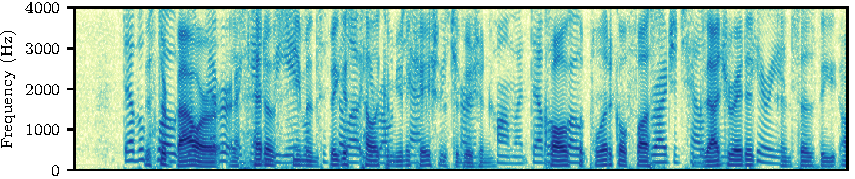
\includegraphics{figure/masking_demonstration-1.pdf}
		\caption{Spectrogram of a mixture in which two persons are talking.}
	\end{subfigure}

	\begin{subfigure}[t]{\textwidth}
		\centering
		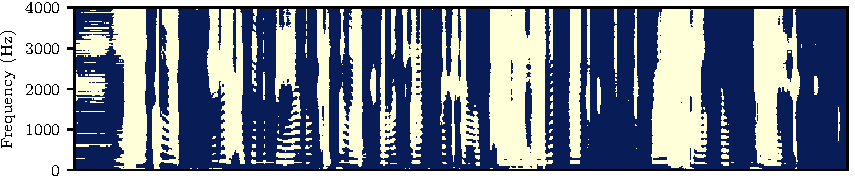
\includegraphics{figure/masking_demonstration-2.pdf}
		\caption{Mask for a single speaker.}
		\label{fig.masking-demonstration.mask}
	\end{subfigure}

	\begin{subfigure}[t]{\textwidth}
		\centering
		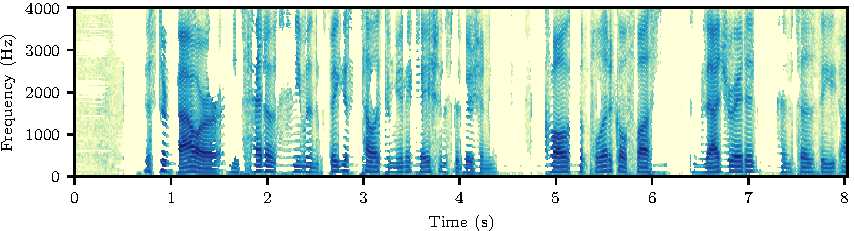
\includegraphics{figure/masking_demonstration-3.pdf}
		\caption{Separated spectrogram, which was created by applying the mask in Figure \ref{fig.masking-demonstration.mask}.}
	\end{subfigure}%
	\caption{Spectrogram of a mixture and a binary mask. The product of the two is shown in the last spectrogram. Dark blue is equal to one whereas the yellow parts correspond to zero.
	Each point corresponds to the power of the given frequency and time. 
	%The scale for the power is left out as only the relative values are meaningful for this example.
	}
	\label{fig.masking-demonstration}
\end{figure}

A formal definition of the speech separation using \gls{dc} is the following: Let $x(n) \in \mathbb{R}$ be the samples of a mixture with $k$ concurrent speakers, where $0 \le n < N$. \acrlong{dc} computes the estimated sources $(x_i)_{i=0}^{i=k}$ such that $\sum_{i=1}^{k}x_i=x$.
The constraint that the sum of the estimated sources must be equal to the mixture is fulfilled by using a mask like the \gls{ibm} (see \ref{def.ibm}).

A \gls{rnn} calculates for each time-frequency bin a vector in a lower dimensional space. This mapping is also called an embedding.
These vectors can be clustered such that the vectors of the same speakers are close together. Using the labels of the clusters it is possible to create an \gls{ibm}. Because vectors of the same speaker should be assigned to the same cluster, the permutation problem is circumvented. As seen in Figure \ref{fig.dc-stages}, the \gls{dc} approach can be structured into multiple stages. We will shortly go over these stages to give an overview of the method according to \cite{Hershey2016}.

\begin{figure}[ht]
	\centering
	\begin{tikzpicture}[node distance = 3cm, label distance=2mm, auto]
		\tikzstyle{block} = [rectangle, draw, text width=6.5em, text centered, rounded corners, minimum height=4em]
		\tikzstyle{line} = [draw, -latex']
		% Place nodes
		\node [block, label=below:Stage 1 (\ref{sec.preprocessing})] (feature) {Feature Extraction};
		\node [block, label=below:Stage 2 (\ref{sec.architecture}), right of=feature] (rnn) {\gls{rnn}};
		\node [block, label=below:Stage 3 (\ref{sec.clustering}), right of=rnn] (clustering) {Clustering};
		\node [block, label=below:{Stage 4 (\ref{sec.clustering}, \ref{sec.reconstruction})}, right of=clustering] (masking) {Creation of Mask};
		\node [block, label=below:Stage 5 (\ref{sec.reconstruction}), right of=masking] (reconstruction) {Waveform Reconstruction};
		% Draw edges
		\path [line] (feature) -- (rnn);
		\path [line] (rnn) -- (clustering);
		\path [line] (clustering) -- (masking);
		\path [line] (masking) -- (reconstruction);
	\end{tikzpicture}
	\caption{The five stages of \acrlong{dc} with references to the sections where they are discussed.}
	\label{fig.dc-stages}
\end{figure}

% Stage 1: Calculate power spectrum
The \textbf{Feature Extraction} stage is responsible for creating the input features for the neural network. The input mixture is transformed to the time-dependent frequency representations using \gls{stft}. For a given discrete input signal $x(n)$ the logarithmic power spectrum is calculated. At this point it is possible to adjust the features using feature engineering. More details on how to further modify the input can be found in Section \ref{sec.preprocessing}.

% Stage 2: Calculate vectors in embedding space
The \textbf{\gls{rnn}} stage calculates for each time-frequency bin a $d$-dimensional vector using a \gls{rnn}. The space of these vectors is also called an embedding space.
The input of the network is a matrix which contains the time-frequency information over a specific time frame.
The output of the network is exactly one $d$-dimensional vector for each time-frequency bin.

% Stage 3: Vector cluster
The \textbf{Clustering} stage determines the centers of the resulting clusters in the embedding space. Lloyd's algorithm is used in order to perform k-means clustering~\cite{Lloyd1982}, as it represents one of the most wildly used algorithm for this task~\cite{Berkhin2002}.
The centers are initialized using k-means++~\cite{Arthur2007}. Clustering can be performed locally or globally. The former means that clustering is performed on the output of the neural network of a single iteration. The latter means that the clustering happens after all embedding vectors of all time-frequency bins have been collected. The difference between these methods will be discussed further in Section \ref{sec.clustering}.

% Stage 4: Calculate and apply mask
In the \textbf{Creation of Mask} stage a mask is calculated by using the label information retrieved from clustering. The \gls{dc} method assumes that in each time-frequency bin exactly one voice is dominant. Therefore, each bin can be assigned to one of $k$ sources. For each speaker $0 \le i < k$ a mask $M_i$ is constructed in such a way that its multiplication with the spectrum of the mixture yields the estimated speech signal of the $i$-th speaker.
One might say that calculating the mask is like adding another dimension to the time-frequency representation. In addition to the time and frequency dimension, a new dimension is added which denotes the belonging to a specific source.

% Stage 5: Reconstruct sprectra
The final stage is the \textbf{Waveform Reconstruction} of the separated spectra. The \gls{dc} method uses only the amplitude information of the \gls{stft}.
In the case of speech the amplitudes are more important than the phase.
Because of that, it is sufficient to use the phase information from the mixture, even though reconstructing the phase could improve the overall performance~\cite[p.11]{Wang2018b}.
To get a discrete signal from the time-frequency representation the inverse \gls{stft} is used.
Apart from numerical errors, there is no error introduced from the inverse \gls{stft} of the unmodified frequency representation from the mixture. Because the window which was used when extracting the features fulfills the \gls{cola} criterion, the numerical errors are negligible.
In conclusion, the quality of the mask is responsible for the success of the source separation.

\section{Expectations of Deep Clustering}\label{sec.expectations}

We will shortly highlight the expectations of the \acrlong{dc} speech separation method. As described Section \ref{sec.challenges} the label permutation problem should be solved. Furthermore, the approach should be able to separate more than 2 speakers. The \gls{dc} approach promises to separate a variable amount of voices from each other. This holds true even when the network is trained on mixtures of two speakers and tested on mixtures with three speakers. The separation also does not depend on knowing the speakers before training. \cite{Hershey2016}

In addition to the mentioned goals the separation should also work on real-world data. This will be evaluated in Chapter \ref{sec.experimental-evaluation} by using different data sets. Mixtures with broadband noise could be difficult to separate because of its presence in a great range of frequency bins. Especially if the noise overlaps with speech in the \SI{4}{\kHz} range, the task becomes more difficult.

As the goals and expectations for the \gls{dc} approach are set we will discuss the method in detail in the following sections. 
The sections \ref{sec.preprocessing}, \ref{sec.architecture}, \ref{sec.clustering} and \ref{sec.reconstruction} deal with the inference of the separated audio signals and assume a trained network. In Section \ref{sec.training} we will discuss how the network should be trained to achieve the expected results.

\section{Pre-processing and Feature Extraction}\label{sec.preprocessing}
Before we define the exact model in Section \ref{sec.architecture} the input features should be discussed. Recall that the input of the network should be a mixture and the output embeddings. In this section we go over the process of preparing a mixture such that it can be fed into the recurrent neural network.

% TODO: Should we use the first and last frequency bin? e.g. 129 eff or 127? Because first one is not independent from the others but the mean

The first step is to load the samples $x(n)$ of the monaural discrete mixture signal for $0 < n < N$. The \gls{dc} method only uses a single channel as described in Chapter \ref{sec.challenges}.
In order to determine the duration of the audio it is required to know the sampling rate $f_s$. The sampling rate is fixed in this paper to $f_s=8\si{\kHz}$. According to the Nyquist sampling theorem this allows a maximum frequency of \SI{4}{\kHz} to be sampled. This maximum frequency offers sufficient intelligibility because the resulting bandwidth is acceptable for vowels spoken by most people~\cite{Heide1998}.
Furthermore, it also limits the amount of computational resources needed~\cite[p.~33]{Hershey2016}.
The duration in seconds of the signal $x$ is given by $N \cdot f_s$.

Next the \gls{stft} needs to be determined which expects the window length $M=256$, hop size $H=0.25M$ and a window function as parameters~\cite{Hershey2016}. In this paper the Hann window function is used like presented in Figure \ref{fig.hann}\footnote{It is assumed that the original paper also uses the Hann window function even though it specifies a squared Hann window. This is due to the common parameter $\alpha=1$ which squares the window function.}.
The notes of Section \ref{sec.foundation-dsp} apply in order to allow a reconstruction using the overlap-add method.
This window length corresponds to a duration of \SI{32}{\ms} and a hop duration of \SI{8}{\ms}.
The spectrum $S(t, m)$ is defined for $0 \le t \le \frac{N-M}{H}$ and $0 \le m \le \frac{M}{2}$. It is assumed $x$ has at least $M$ samples.
% (M/2)+1 bins is correct. (N-M) / H + 1 windows is correct

At this point it is required to make sure that the spectrum does not contain zeroes by calculating $S_+(t, m) = \max(|S(t, m)|, \epsilon)$, where $\epsilon=1e-10$ is a constant which denotes the minimal magnitude.
This allows the definition of the power spectrum according to Equation \ref{eq.decibel}:
\begin{equation}
	S_{pwr}(t,m)=20\log_{10}(S_+(t, m))\,\si{\dB}.
\end{equation}
In Section \ref{sec.foundation-dsp} it was noted that the signal should be scaled in order to recover energy which is lost due to windowing or missing negative frequencies.
This is not required here because the scaling of the input does not influence the performance of the network.

% VAD
\label{paragraph.vad}
A beneficial step is to apply \gls{vad}, which allows discarding quiet segments which are not important for the separation procedure. \gls{vad} is a common pre-processing step and can be done in time-domain and frequency domain~\cite{Adiga2016}. Because we already operate in the frequency domain, it is straight forward to do it in this domain. A simple approach is to define a binary mask $\mathrm{VAD}(t,m)$ which defines which time-frequency bin is active and which is not. Active means that the power of that bin is above a certain threshold. The threshold can be chosen to be $40\,\si{\dB}$ below the maximum value of the power spectrum.

% mean and std
Furthermore, normalization of the mixture is a beneficial step. The neural network input is normalized according the mean $\mu$ and standard deviation $\sigma$ of the training data set which is determined according to the process in Section \ref{sec.preparing-datasets}. Using the definition of the standard score~\cite[p.~1018]{Kreyszig2006}
\begin{equation}
	\hat{X}(t,m)=\frac{X(t,m)-\mu}{\sigma}
	\label{eq.standard-score}
\end{equation}
it is possible to normalize the values of the time-frequency spectrum $S_{pwr}(t, m)$.

% Output
Last the time-frequency power spectrum is segmented into frames where each frame has a specific maximum amount of windows $\#_w$. This is due to the limited amount of data a \gls{rnn} is able to process at once. In Section \ref{fig.rnn} the input matrix $I$ was mentioned which contains the feature vectors. The matrix for the first frame is
\begin{equation*}
	I=
	\begin{pmatrix}
		S_{pwr}(0, 0)    & S_{pwr}(0, 1)    & \ldots & S_{pwr}(0, \frac{M}{2})    \\
		S_{pwr}(1, 0)    & S_{pwr}(1, 1)    & \ldots & S_{pwr}(1, \frac{M}{2})    \\
		\ldots           & \ldots           & \ldots & \ldots                     \\
		S_{pwr}(\#_w, 0) & S_{pwr}(\#_w, 1) & \ldots & S_{pwr}(\#_w, \frac{M}{2}) \\
	\end{pmatrix}.
	\label{eq.input-for-network}
\end{equation*}

An important constant is the batch size $b_s$ which was already mentioned in \ref{sec.mlp-backpropagation}. During training $b_s$ matrices are fed into the neural network at once. During the testing phase the batch size is expected to be one, as we want the outputs for a single frame.

\section{Network Architecture}\label{sec.architecture}

As already described in the beginning of the chapter the goal of the recurrent network in \gls{dc} is to determine a $d$-dimensional vector for each time-frequency bin.
The network architecture makes use of 2 bidirectional \gls{lstm} layers and a single feedforward layer with $\tanh$ as activation function. The paper by~\textcite[p.~33]{Hershey2016} also evaluates the logistic function but no significant difference was found in the performance of the method.
In contrast to \gls{lstm} cells, there is also the possibility to use \gls{gru} cells. They offer a simpler model and lacks for example an output gate~\cite{Chung2014}. \textcite{Chung2014} showed empirically that the performance in on pair for specific tasks. The results in Section \ref{sec.training} show that using an \gls{lstm} network is beneficial for \gls{dc}.
Furthermore, dropouts are applied to the forward and backward layers of the \gls{rnn} like discussed in Section \ref{sec.training}.

% Is there a way to write layer transformations more fluent?
The actual input $I_{b_s}$ of the neural network is a $b_s \times \#_w \times \frac{M}{2}+1$ matrix. Each batch has $b_s$ frames where each frame has $\#_w$ windows according to Equation \ref{eq.input-for-network}. The duration of such a frame is approximately \SI{824}{\ms} which is about the length of a spoken word~\cite[p.~33]{Hershey2016}. % (100-1) *(64) + 256) / 8000 = 824
Each window holds the $\frac{M}{2}+1$ frequency bins. The matrix $I_{b_s}$ has the correct shape to be an input of a recurrent \gls{lstm} layer.

The output of the bidirectional layers are concatenated and reshaped such that they can be input for the final feedforward layer. After concatenating and reshaping the output of the bidirectional layer it has the shape $q \times 2 \cdot 600$, where $q=b_s \#_w$. The output of the feedforward layer has the shape $q \times (\frac{M}{2}+1) d$ which is reshaped to a $p \times d$ matrix, where $p=q(\frac{M}{2}+1)$.
For $0 \le i < p$ each $d$-dimensional vector $v_i$ is normalized in a last step such that:
\begin{equation}
	|v_i|^2=\sum_{i=0}^{d-1} v_i^2=1,
\end{equation}
where $|.|$ is the Euclidean norm.

Therefore, the final matrix $V \in \mathbb{R}^{p \times d}$ assigns each of the $p$ time-frequency bins a normalized $d$-dimensional vector.
The matrix $VV\tran \in \mathbb{R}^{p \times p}$ is called the estimated affinity matrix. When training the network, the weights will be optimized such that the estimated affinity matrix is most similar to the ideal binary affinity matrix $YY\tran$. What the training target $YY\tran$ means and why it is important for the success of the clustering is explained in the next section.

\subsection{Loss Function}\label{sec.loss-dc}

The training target of the neural network is the ideal affinity matrix $YY\tran \in \mathbb{R}^{p \times p}$, where $p$ is the amount of frequency bins which should be assigned to one of $k$ speakers.

This matrix is created from a target partition $Y \in \mathbb{R}^{p \times k}$ which is known during training. For $0 \le i < p$ and  $0 \le j < k$ the value of $y_{ij}$ is defined to be the $j$-th element of the $i$-th row of $Y$.
That value belongs to the cluster $j$ and therefore to the speaker $j$ if and only if $y_{ij}$ is equal to 1. The vector $y_i=\begin{psmallmatrix}y_{i,0} & y_{i,1} & \ldots & y_{i,k-1}\end{psmallmatrix}$ is a one-hot vector which has a 1 at the index which denotes the cluster belonging. The multiplication with its transpose yields an affinity matrix with an interesting property. For $0 \le i,j < p$ the element $(YY\tran)_{ij}$ is equal to 1 if the bins $i$ and $k$ belong to the same cluster and 0 if otherwise. Therefore, the affinity matrix is a symmetric square matrix of size $p$, where the diagonal consists only of ones.

% Definition
With that knowledge it is possible to define a loss function $J$ which reaches zero when the $p \times p$ estimated and ideal affinity matrices $VV\tran$ and $YY\tran$ are equal:
\begin{equation}
	\begin{split}\label{eq.loss}
		J(Y, V) & = || VV\tran - YY\tran ||^2_F \\
				& = \sum_{\substack{i=0,j=0 \\ y_i = y_j}} \left(| v_i - v_j |^2 - 1)\right) + \sum_{i=0,j=0} (v_i\tran v_j)^2
	\end{split},
\end{equation}
where $|| . ||^2_F$ is the squared Frobenius norm which sums over the squared difference between the entries of the matrices. The transformation into two terms can be reviewed in Appendix \ref{appendix.loss-descriptive}. In Equation \ref{eq.loss} the first term is directly related with the k-means objective from Equation \ref{eq.k-means-objective} and pulls the embeddings of the same speakers together. The second term spreads the vectors apart and thus avoids trivial solutions~\cite[p.~32]{Hershey2016}.

This means if the loss is small when the k-means algorithm is able to reach a small $\gamma$ on the embeddings in $V$.

To summarize, if the network is trained properly (see Chapter \ref{sec.training}) such that the difference between $VV\tran$ and $YY\tran$ is small then the calculated embeddings $v_i$ and $v_j$ have a small distance if they belong to the same speaker.

It is noteworthy that the $p \times p$ matrices $VV\tran$ and $YY\tran$ are constructed in two different ways. In the former case the matrix $V$ consists of $p$ embeddings. In the latter case $Y$ consists of $p$ one-hot vectors which denote the speaker belonging.
In each case the multiplication by its transpose yields two matrices which can be compared.

The label permutation problem which was mentioned in Section \ref{sec.challenges.label-permutation} is circumvented here because embeddings from the same speaker will always have a small distance to each other. By using the presented loss function the neural network doesn't learn which frequency bin belongs to which speaker but only learns to put vectors from the same speaker close together in the embedding space.

The loss function in Equation \ref{eq.loss} consumes quite a lot of memory because $p \times p$ matrices are constructed. A matrix which contains the time-frequency bins for 100 windows would already have $166 \cdot 10^6$ entries.
Fortunately, an efficient implementation exists which exploits the fact that the objective has a low rank:
\begin{equation}
	J(Y, V) = || V\tran V ||^2_F - 2 || V\tran Y||^2_F + || Y\tran Y||^2_F
	\label{eq.loss-fast}
\end{equation}
where $V\tran V$ is a $d \times d$, $V\tran Y$ a $d \times k$ and $Y\tran Y$ a $k \times k$ matrix \cite[p. 32]{Hershey2016}. A proof for this transformation can be found in Appendix~\ref{appendix.loss-fast}.
It's derivative is given by:
\begin{equation}
	\frac{\partial J}{\partial V\tran} = 4V(V\tran V) - 4Y(Y\tran V).
\end{equation}

In conclusion, the neural network is able to generate an embedding for each time-frequency bin, which has the property that other embeddings originating from the same speaker have a small Euclidean distance. This fact enables us to create clusters from these embeddings, which will be exploited in Section \ref{sec.clustering}.

\subsection{Frequency Mask as Training Target}\label{sec.masks}

% Embedding-based training target
When training a neural network in a supervised manner it is essential to define a proper training target. In the last section a training target was introduced which maps each time-frequency bin to a vector in embedding space. We will refer to this training target as being embedding-based.

There are two other categories of training targets, namely mapping-based and masking-based targets~\cite{Wang2018b}. In the first case the spectral time-frequency representation of the separated sources is directly used. A masking-based target in contrast, calculates the belongings of each time-frequency bin to a specific estimated source. The Definition \ref{def.ibm} will be used in this thesis whenever we speak about a mask.

\begin{definition}{Ideal Binary Mask}
	The Ideal Binary Mask defines which time-frequency bin belongs to which source in a mixture. For the power spectra $X_{pwr}$ and $Y_{pwr}$ the mask is defined as~\cite[p.~187]{Wang2005}:

	\begin{center} % Should I have the X,Y in the indices?
		$\mathrm{IBM}(t,m)=
			\begin{cases*}
				1 			& if $X_{pwr}(t,m) > Y_{pwr}(t,m)$ \\
				0        	& otherwise
			\end{cases*}$.
	\end{center}
	\label{def.ibm}
\end{definition}

The \gls{ibm} is 1 for each time-frequency bin in which the power in the spectrum $X$ dominates the power in $Y$. One might also say that the \gls{ibm} is 1 for each time-frequency bin where the \gls{snr} defined as $\frac{X_{pwr}}{Y_{pwr}}$ is above the 0\si{\dB} threshold.

Amongst other masks~\textcite[p.~5]{Wang2018b} also introduce the ideal ratio mask and its complex version as a training target. They can be seen as a soft version of the \gls{ibm}. The complex mask allows the neural network to estimate the phases as well~\cite{Williamson2016}. This motivation arises from an evaluation which claims that the phase has an impact on the quality of speech~\cite{Paliwal2011}. Nonetheless, the \gls{ibm} is seen as sufficient for the needs of \gls{dc}~\cite{Hershey2016}.

We pointed out two other training targets shortly in this section in order to introduce the \gls{ibm}. The target of the next section is to create a similar mask using a clustering algorithm which is able to separate more than two sources.

\section{Clustering in the Embedding Space}\label{sec.clustering}

As already described in Figure \ref{fig.dc-stages} the \acrlong{dc} method has multiple stages. In the last two sections the pre-processing and neural network model were covered. These are responsible for the term \textit{Deep}. We explore now the second major part which is the \textit{Clustering}.

The k-means algorithm which was introduced in Section \ref{sec.k-means} is used to perform the clustering. The properties of the embedding vectors in $V$ have been discussed in the last section. The clustering of these vectors will lead to a result which determines which time frequency bin belongs to which speaker. In this section the process of k-means clustering is formalized in a way that allows a formal definition using matrices..

\textcite{Hershey2016} introduce the clustering as a matrix factorization problem~\cite{Bauckhage2015}. The objective function of Equation \ref{eq.k-means-objective} can be reshaped as:
\begin{equation}
	\gamma=\sum_{i=0}^{p} \sum_{j=0}^{k} z_{ij} ||v_i - c_j||^2,
	\label{eq.k-means-objective-binary}
\end{equation}
where
$v_i \in \mathbb{R}^d$ is an embedding vector of $V$,
$c_j \in \mathbb{R}^d$ is a centroid vector of the $k \times d$ matrix $M$ and
\begin{equation*}
	z_{ij}=\begin{cases*}
		1 			& if $x_i \in \mathcal{K}_j$ \\
		0        	& otherwise
	\end{cases*}
\end{equation*}
is a binary entry of the $p \times k$ matrix $Z$. The Equation \ref{eq.k-means-objective-binary} is in fact equal to Equation \ref{eq.k-means-objective} because the cluster $\mathcal{K}_j$ is defined to be a set of data points which are closest to the center $c_j$, where $0 \le j < k$ is the index of the cluster. Equation \ref{eq.k-means-objective-binary} can be expressed using the Frobenius norm:
\begin{equation}
	\gamma=||V-ZM||_F^2,
\end{equation}
where $M=(Y\tran Y)^{-1}Y\tran V$~\cite{Bauckhage2015}.
The objective remains to minimize $\gamma$. The notation using matrices allows a more compact way of defining the problem.
Furthermore, it allows to calculate the success of the clustering after applying the k-means algorithm.
The squared error between the estimated frequency cluster assignments $Z$ and the true labels $Y$, which both have the shape $p \times k$, can be defined in the following way \cite[p. 32]{Hershey2016}:
\begin{equation}
	d(Y, Z)=||Y(Y\tran Y)^{-1} Y\tran  -  Z(Z\tran Z)^{-1} Z\tran ||_F^2.
\end{equation}

The process from estimating the embedding vectors to clustering the vectors using k-means is determined by the several objectives. The training objective $J(Y, V)$, the k-means objective $\gamma$ and the clustering error $d(Y, Z)$ are small, if $VV\tran \approx YY\tran$ which leads to $Z \approx Y$\cite[p. 33]{Hershey2016}.

% The number of speakers not fixed
In the introduction of this thesis the challenge of separating an arbitrary count of different voices was mentioned (see Section \ref{sec.challenges}). As shown in experiments the \gls{dc} approach is able to generalize to more than one voice, even when trained on only two~\cite[p.~34]{Hershey2016}. The proposed structure allows this by using a parameter $k>2$ when clustering with k-means, without changing the loss function $J$.

The dimension of the matrix $Z \in \mathbb{R}^{p \times k}$ reminds of the already mentioned concept of a binary mask. And indeed, the matrix is nothing else than a binary mask which is defined as:
\begin{equation}
	\mathrm{IBM}(t,m, j)=z_{t(\frac{M}{2}+1)+m,j},
	\label{eq.ibm-final}
\end{equation}
where $i$ corresponds to the speaker $0 \le j < k$.
In this thesis we will focus on the separation of two speakers such that $i \in \{0,1\}$.
This mask will be used in Section \ref{sec.reconstruction} to construct the estimated sources of the mixture.

Lastly, there are two different ways of doing the clustering. The way it was described so far is called local clustering because the output $V$ is clustered directly. The other way is called global clustering. The outputs of the neural network are concatenated and stored in order to do the clustering, once the end of the input signal $x$ has been reached. Experimental evaluations show that the local clustering which is used in this thesis performs slightly better~\cite[p.~34]{Hershey2016}.

The next section covers the final stage which deals with the reconstruction of estimated source signals in the time-domain.

\section{Reconstructing the Waveform}\label{sec.reconstruction}

% Adding another dimension to the DFT (the mask)
The previous sections explained in detail how to compute a binary mask staring from the time domain representation of the discrete signal $x$. This process added another dimension to the \gls{stft}. Apart from the two dimensions for time and frequency a third one was added which denotes the speaker belonging.

Finally it is possible to create the estimated output signal $\tilde{x}^i$, where $0 \le i < k$ is the index of the speaker we wish to isolate.
As defined in Section \ref{sec.preprocessing} the complex \gls{stft} of the mixture is $S(t,f)$. In Equation \ref{eq.ibm-final} the final \gls{ibm} is defined.
The first step is to create a modification $\tilde{S}^i(t,f)$ of the \gls{stft} of the mixture for each speaker $i$:
\begin{equation}
	\tilde{S}^i(t,f)=\mathrm{IBM}(t,f,i) \cdot S^i(t,f),
\end{equation}
where $\cdot$ multiplies the real part of $S^i(t,f) \in \mathbb{C}$ by $\mathrm{IBM}(t,f,i) \in \mathbb{R}$ and leaves the phases untouched.
The \gls{dc} approach only reconstructs the magnitudes for the estimated signals. Therefore, the phases are taken from the mixture.
The next step is to inverse the \gls{stft} $\tilde{S}^i(t,f)$ using the overlap-add approach. As described in Section \ref{sec.foundation-dsp} a padding at the start and end is required such that no information is ignored because of windowing as indicated by Figure \ref{fig.hann-summed}.
Because of the interaction between the Hann window function, overlapping and padding in the overlap-add method nearly perfect reconstruction is possible.
The inverse \gls{stft} creates a time discrete signal $\tilde{x}^i$ for each speaker $i$.

We finished now the fifth stage of the \gls{dc} approach and acquired estimated source signals which are close to the reference signals. The next chapter describes how estimated sources can be compared to the references in order to measure performance when training the network in different ways.

\chapter{Experiments}\label{sec.experimental-evaluation}

Chapter \ref{chapter.dc} covered how the separation works given that the neural network performs well. In this chapter a visualization of the embedding space is shown in order to illustrate the \gls{dc} approach. 
Furthermore, the amount of concurrently speaking persons is determined experimentally in Section \ref{sec.order-selection}.
Lastly, the training of the network is discussed in order to achieve good results. The training of a neural network adjusts a great amount of parameters. Nonetheless, hyper-parameters exist which require manual adjustment. The assembly of the data set also determines the performance of the separation approach and requires discussion.

\section{Visualization of Vectors in the Embedding Space}

As defined in Section \ref{sec.k-means}, the output of the k-means algorithm is a set of $k$ clusters $\mathcal{K}=\{\mathcal{K}_0, \mathcal{K}_1, \ldots, \mathcal{K}_{k-1}\}$. 
The vectors in the clusters are $d$-dimensional. 
As in most cases the dimension of the embeddings is greater than 10~\cite[p.~34]{Hershey2016}, it is impracticable to visualize the clustering directly.

This ''curse of dimensionality''~\cite{Keogh2017} led to algorithms which reduce the dimensionality of the data. There are mainly two ways of performing the reduction. Firstly, there is feature selection which selects the ''best'' subset of the $d$ dimensions. The best subset depends on the task and data.
On the contrary, feature extraction transforms the original vector to create new feature vector with a lower dimensionality.~\cite[p.~103]{Pudil1998}

We will focus on the visualization using \gls{pca} which transforms the vectors in the rows of $V$ to vectors of dimension $L$. \gls{pca} is restricted in a sense such that the computed features are a linear combination of its basis vectors. Therefore, \gls{pca} basically changes the basis of the input data.~\cite[p.~3]{Shlens2014}

\begin{figure}
	\centering
	\begin{subfigure}{0.5\textwidth}
		\centering
		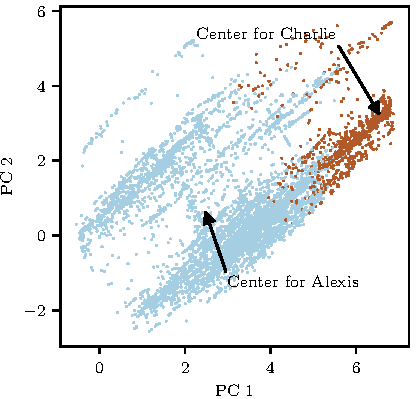
\includegraphics{figure/pca/pca0.pdf}
	\end{subfigure}%
	\begin{subfigure}{0.5\textwidth}
		\centering
		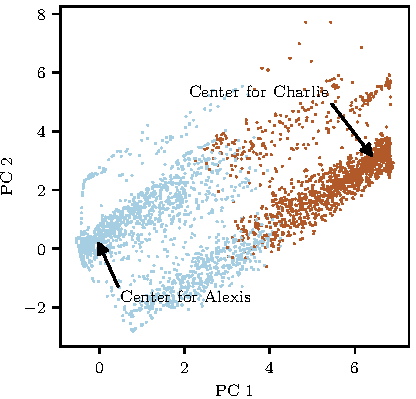
\includegraphics{figure/pca/pca1.pdf}
	\end{subfigure}%
	\vskip\baselineskip
	\begin{subfigure}{0.5\textwidth}
		\centering
		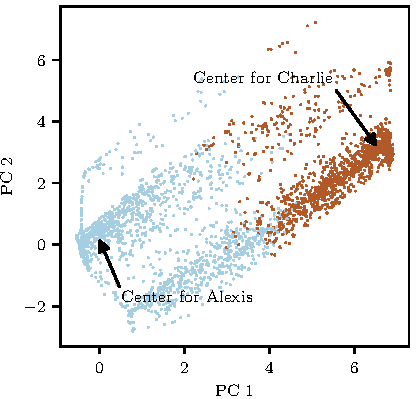
\includegraphics{figure/pca/pca7.pdf}
	\end{subfigure}%
	\begin{subfigure}{0.5\textwidth}
		\centering
		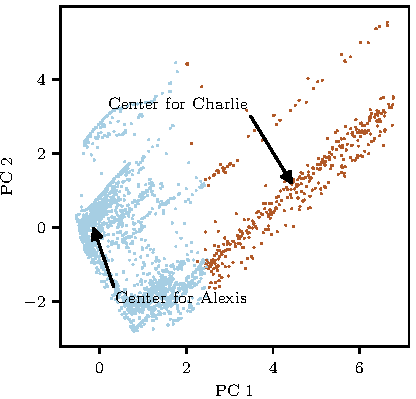
\includegraphics{figure/pca/pca10.pdf}
	\end{subfigure}%
	\caption{\gls{pca} of four frames with each $\#_w (\frac{M}{2}+1)$ data points using two components. Each point represents a single embedding vector.
	The arrows point to the center of mass of the two clusters. Each center correspond to the voice of a specific speaker like Alexis or Charlie. It is clearly visible that the loss function tries to pull certain embeddings closer together. According to Equation \ref{eq.loss} vectors which are close together belong to the same speaker.
	The frames are selected from a signal which is longer than four frames. The first and the last frame stand out as Alexis and Charlie just started talking or already stopped.}
	\label{fig.clustering-pca}
\end{figure}

Apart from being pretty the visualization can help to identify implementation errors. For example if the center of the cluster for ''Alexis'' in Figure \ref{fig.clustering-pca} is shown on the right instead of the left for some time steps, then the cluster labels are confused.

In essence such a visualization gives a good intuition what the output of the neural network means. It can also identify a malfunctioning network if the \gls{pca} fails and no clusters are identifiable.

\section{Clustering Order Selection}\label{sec.order-selection}

When dealing with long recordings of multiple speakers talking at the same time, it is likely that speakers appear and disappear. In this section we try to estimate at which time there are two speakers or only a single speaker.

The resolution of the estimation is one frame which corresponds to 100 overlapping windows. For each approximately \SI{0.8}{\second} frame, k-means clustering is performed with different values for $k$. The example audio is the concatenation of several utterances. In the first part only one person is speaking, in the second two, in the third again one and in the last two. This signal is investigated using a metric of distance and clustering score.

In Figure \ref{fig.order-selection.centers} the fact that the loss objective (see Section  \ref{sec.loss-dc}) pushes embeddings apart which belong to different speakers is exploited. For $k=1$ the plot shows the Euclidean distance from the origin to the center of mass of the embeddings. For $k=2$ the red plot shows the Euclidean distance between the two centers.
It is possible to observe that the distance between the centers is low if only a single person is talking. As soon as a speaker appears the centers are pushed apart.
Furthermore, when clustering with $k=1$ the center is further apart from the origin if the $k$ matches the count of speakers. 

\begin{figure}[ht]
	\begin{subfigure}[t]{0.48\textwidth}
		\centering
		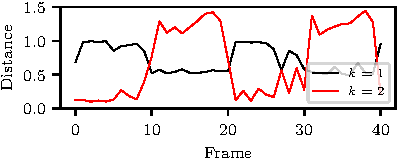
\includegraphics{figure/elbow/centers_1.pdf}
	\end{subfigure}
	\begin{subfigure}[t]{0.48\textwidth}
		\centering
		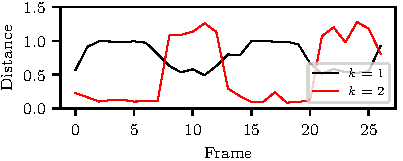
\includegraphics{figure/elbow/centers_2.pdf}
	\end{subfigure}%
	\caption{The plots show the Euclidean distance between the origin and the center for $k=1$, as well as the distance between the two clusters for $k=2$. In each audio signal the first segment contains one voice, the second two, the third again one and the last two.}
	\label{fig.order-selection.centers}
\end{figure}

Another way to look at the clustering is by using the objective of k-means which tries to minimize the \gls{wce}. Figure \ref{fig.order-selection.scores} shows the error for each frame and for $k=1$ and $k=2$. In the second and fourth segment in which two voices are present the error for $k=2$ is lower than that compared to $k=1$.
This means using k-means clustering with $k=2$ yields a lower error and therefore is the correct choice. The observations hold true for various speakers and voices.

\begin{figure}[ht]
	\begin{subfigure}[t]{0.48\textwidth}
		\centering
		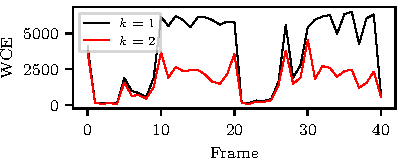
\includegraphics{figure/elbow/scores_1.pdf}
	\end{subfigure}
	\begin{subfigure}[t]{0.48\textwidth}
		\centering
		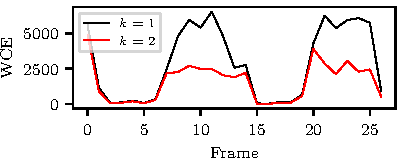
\includegraphics{figure/elbow/scores_2.pdf}
	\end{subfigure}%
	\caption{The \gls{wce} of two audio signals consisting of four segments over time. The signals consists of four segments like described in Figure \ref{fig.order-selection.centers}.}
	\label{fig.order-selection.scores}
\end{figure}

Unfortunately this the two proposed methods only showed success for differentiating between a single and multiple speakers. As soon as it is attempted to distinguish between two and three speakers the proposed methods fail. The average distance between the centers for $k=3$ is very similar to the distance between the centers for $k=2$. Furthermore, the \gls{wce} is also very similar for $k=2$ and $k=3$.

This section showed another way of visualizing the results of the clustering by comparing the results over time for different orders. In summary we can be confident that the algorithm achieves its goal of separating voices. 
In order to prove this experimentally, the next step is to establish a performance criterion to compare the approaches and data sets.

\section{Evaluation metrics}\label{sec.method-selection}
When comparing earlier approaches like those mentioned in Section \ref{sec.approaches}  or new methods with each other an objective metric for the success of the separation is required. Even though subjective studies like in Figure \ref{fig.intelligibility} can evaluate the intelligibility of the separated speech, they are expensive to conduct. Furthermore, a subjective evaluation does not offer good comparability.
Therefore, in \citeyear{Vincent2006} \citeauthor{Vincent2006} introduced a method for evaluating the performance of speech separation. This measurement is further adopted in \cite{Vincent2007} and \cite{Vincent2012}. 
The metric is actually defined for audio with more than one channel like stereo recordings. Because of that the term spatial image is introduced. In this case each channel
\begin{equation}
	x_i(t)=\sum_{j=0}^{k} s_{ij}^{img}(t),
\end{equation}
yields multiple spatial images which denote the reference sources \cite[p. 3]{Vincent2007}:
In this Equation $x_i(t)$ is the signal of the mixture for channel $i$, $k$ the amount of sources and $s_{ij}^{img}$ the spatial images. As we separate monaural audio this can be simplified to:
\begin{equation}
	x(t)=\sum_{j=0}^{k} s_{j}^{img}(t),
	\label{eq.metric.ref-source}
\end{equation}
where $x(t)$ is the mixture and $s_{j}^{img}(t)$ the signal for the reference source of speaker $j$.
It is noteworthy, that compared to earlier performance measurement methods the proposed method offers multiple criteria, namely the \gls{sir}, \gls{sar}, \gls{isr} and the \gls{sdr} which combines the others.

In order to apply the metric the reference sources and the estimated sources are required. The metric decomposes the estimated source for speaker $j$ as:
\begin{equation}
	\hat{s}_{j}^{img}(t) = s_{j}^{img}(t) + e^{spat}_{j}(t) + e^{interf}_{j}(t) + e^{artif}_{j}(t),
\end{equation}
where the error terms $e^{spat}_{j}(t)$, $e^{interf}_{j}(t)$ and $e^{artif}_{j}(t)$ represent the spatial distortion, interference and artifacts, $s_{j}^{img}(t)$ the reference source as introduced in Equation \ref{eq.metric.ref-source} and $\hat{s}_{j}^{img}(t)$ the estimated source~\cite{Vincent2012}. The final metric in terms of ratios is defined as:
\begin{equation}
	\mathrm{ISR}_j=10\log_{10}{
	\frac{\sum_{t}s_{j}^{img}(t)^2}
	{\sum_{t}e_{j}^{spat}(t)^2}},
	\label{eq.isr}
\end{equation}
\begin{equation}
	\mathrm{SIR}_j=10\log_{10}{
	\frac{\sum_{t}(s_{j}^{img}(t)+e_{j}^{spat}(t))^2}
	{\sum_{t}e_{j}^{interf}(t)^2}},
	\label{eq.sir}
\end{equation}
and:
\begin{equation}
	\mathrm{SAR}_j=10\log_{10}{
	\frac{\sum_{t}(s_{j}^{img}(t)+e_{j}^{spat}(t)+e_{j}^{interf}(t))^2}
	{\sum_{t}e_{j}^{artif}(t)^2}}.
	\label{eq.sar}
\end{equation}
The combined metric is defined as:
\begin{equation}
	\mathrm{SDR}_j=10\log_{10}{
	\frac{\sum_{t}s_{j}^{img}(t)^2}
	{\sum_{t}(e_{j}^{spat}(t)+e_{j}^{interf}(t)+e_{j}^{artif}(t))^2}}.
	\label{eq.sdr}
\end{equation}

In most cases it is not possible to know which estimated source corresponds to which reference source as their order is arbitrary due to the label permutation problem. Therefore the estimated sources have to be matched to their reference. This is done by testing the each permutation and taking the result which yields the lowest \gls{isr}~\cite[p. 5]{Vincent2012}.

\textcite[p. 5]{Vincent2007} note that depending on the application the error should be weighted differently. For example in hearing aids some interference is acceptable as long as the \gls{sar} is low. For other applications the interference error could be the most important. Therefore the measurement is arbitrary in a sense that it treats all errors equally. 

Although other metrics like PESQ~\cite{Rix2001}, PEASS~\cite{Emiya2011} and STOI~\cite{Taal2010} exist,
the proposed metric is used throughout this chapter in order to evaluate the performance of the \gls{dc} method. The reason for this is that the implementation in the \texttt{BSS Eval} toolkit \cite{Fevotte2005} is used in a lot of papers and therefore offers comparability.
% TODO: SI-SDR and critique
The next sections cover the data and which knobs can be adjusted in order to perform experiments.

\section{Data Sets: TIMIT, WSJ0 and TEDLIUM}\label{sec.datasets}
The choice of the data set and the way how the features are prepared matters a lot in data-driven applications like \gls{dc}. The latter is also known as feature engineering. % TODO: Cite feature engineering
The training and also evaluation of the approach requires on the one hand a mixtures and on the other hand clean reference signals which yield the mixed signal. This is achieved by using raw speech data sets which consist of recordings of single persons talking and mixing them together.

This advantage is unique to the separation of speech. The separation of lead and companion in music raises a greater issue because of the unavailability of reference data. Another noteworthy fact is that the recordings of the individual tracks as well as the mixture undergo post-processing which makes it difficult to create data sets for that use case.~\cite[p.~14]{Rafii2018}

In this section three raw data sets are presented which are used to train, adjust and evaluate the \gls{rnn}. Whereas TIMIT~\cite{Garofolo1993} and WJS0~\cite{Garofolo1994} are not freely available the last one TEDLIUM3~\cite{Hernandez2018} is.
After that the preparation and mixing of the raw data sets is described in Section \ref{sec.preparing-datasets}.

% https://catalog.ldc.upenn.edu/docs/LDC93S1/timit.readme.html
The TIMIT data set consists of utterances spoken by 630 English-speaking individuals with diverse dialects of which 30\% are female and 70\% male. Ten unique sentences are recorded from each speaker which yields 6300 utterances. This data set was recorded under laboratory conditions and therefore offers clean speech signals.~\cite[Documentation]{Garofolo1993}

The summed duration of the utterances is approximately 5.5 hours which makes this a rather small but diverse set because of the great amount of speakers.

% https://catalog.ldc.upenn.edu/docs/LDC93S6A/csrnov92.html
The WSJ0 data set is distributed on several disks. The first 12 compact disks contain training and development material and the last three test data and documentation. Furthermore, the data is subdivided into sets with specific characteristics. For training and adjusting the network the set
\texttt{SI\_TR\_S} (Speaker-Independent Training Spontaneous Dictation) % 8825.458500 + 89689.786375
is used, whereas for evaluation the sets
\texttt{SI\_ET\_05} (Speaker-Independent Evaluation 5K Vocabulary) % 5340.932000 + 5340.932000
and
\texttt{SI\_DT\_05} (Speaker-Independent Development 5K Vocabulary) % 8071.120375 + 
are used. This distribution is the same as in~\cite{Hershey2016}. The recording under laboratory conditions was performed using different kinds of microphones. For the training mostly a close-talking microphone is utilized while for the other sets primarily microphones of varying types are used.
The evaluation data and development set is spoken by 11 men and 9 females. The training set contains utterances from 64 men and 65 women. All speakers are English~\cite[Documentation and speaker information]{Garofolo1994}

The sets used for training and adjustment offer \SI{25}{h} of audio and the set for evaluation approximately \SI{5}{h}.

The TEDLIUM data set is a free\footnote{Licensed under CC BY-NC-ND 3.0} audio collection of 2351 TED talks. The total duration of the audio is \SI{452}{h} of which 69.9\% is from males and 29.6\% from females.~\cite{Hernandez2018}

Unfortunately, no official gender data for individual talks is available for the data set. Furthermore, as the audio is from public talks, background noise from the audience or audio-visual presentations is expected.

All three data sets only offer monaural audio with a sampling rate of \SI{16}{\kHz} which is enough for this application because the separation only uses a single channel and the audio is resampled to a rate of \SI{8}{\kHz} (see \ref{sec.preparing-datasets}).
The waveforms of the data sets are compressed and packed using the NIST \gls{sphere} toolkit. Several tools exist in order to convert them to \gls{riff} waveform audio files in order to allow easy and universal playback and processing. The file header of the \gls{sphere} files offer benefits like a specification of the microphone, recording location or recording session which are not required in the use case of audio separation.


\section{Preparing the Data Sets}\label{sec.preparing-datasets}

\begin{table}
	\centering
	\begin{tabularx}{.8\textwidth}{cXcccc}
		id & data set    & source  & \multicolumn{2}{c}{duration in h} & reference 	\tabularnewline
		   &             &         & T                                 & E                         & \tabularnewline
		\midrule
		A  & TIMIT-mix   & TIMIT   & 30                                & 5                         & \cite{Garofolo1993} \tabularnewline
		\midrule
		B  & WSJ0-mix    & WSJ0    & 30                                & 5                         & \cite{Garofolo1994} \tabularnewline
		\midrule
		C  & TEDLIUM-mix & TEDLIUM & 30                                & 5                         & \cite{Hernandez2018} \tabularnewline
	\end{tabularx}
	\caption{Overview of the data sets used for training. The duration column specifies the amount of training and evaluation data respectively.}
	\label{table.datasets}
\end{table}

The creation of the data set is one of the main tasks in data-driven applications. In this section the process of creating the data sets TIMIT-mix, WSJ0-mix and TEDLIUM-mix like specified in Table \ref{table.datasets} is presented. Every data set is split into two subsets for specific applications. The training set is used to adjust the weights of the neural network. In contrast, the evaluation set, which is also called the test set, is used to measure the performance of the network and its final accuracy.
The training and evaluation using different data sets gives insight whether the hyper-parameterized algorithm adapts to different data.

% Resampling
Depending on the format of the raw data sets specific tasks are needed to create the mixture sets. The first step is to resample and convert the \gls{sphere} files using FFMPEG version 4.1.3 to the rate already mentioned in the last section.

Thereafter, the sets are split into subsets randomly.
For TIMIT the whole set is divided into a training and evaluation set which hold 90\% and 10\% of the data respectively.
For TEDLIUM only the upper 20\% of the longest talks are used. Those 236 talks are split like the TIMIT set.
For WSJ0 \texttt{SI\_TR\_S} is used for training whereas \texttt{SI\_ET\_05} and \texttt{SI\_DR\_05} are used for evaluation.
Within each split speakers are selected such that half of them are female in order to have a diversity in speech. In the case of TEDLIUM, which has no gender data available, speakers are selected randomly and assigned to a split until the percentages of the split match with the constraint that half of the speakers are female.

% Clipping
% TODO: Use the segmentation information from TEDLIUM to remove silences applause
The 236 talks of the test and evaluation set from TEDLIUM have a mean duration of approximately \SI{22}{min}.
Therefore, it is required to create short audio clips from the long TED talks. This is done by randomly selecting 200 \SI{5}{s} audio clips for each speaker from the training set. For the evaluation set only 100 utterances per speaker are created. The first and last \SI{20}{s} are excluded because they usually contain noise from the audience.
The other two data sets already contain short utterances and therefore no action is required.

% Packing
To summarize, we have now three data sets which contain a subset for training and evaluation. Each subset contains utterances with a fair gender distribution. 
For each training set the mean $\mu$ and standard deviation $\sigma$ is determined in order to calculate the standard score like defined in Equation \ref{eq.standard-score}.
This is used in Section \ref{sec.preprocessing} to scale the input features of the neural network.
The last step it to create mixtures from the utterances as well as a matrix $Y$ for each mixture which are required during the training of \gls{dc} (see Section \ref{sec.loss-dc}).

Finally, to create the data sets TIMIT-mix, WSJ0-mix and TEDLIUM-mix, mixtures are generated randomly. This means a random utterance from a random speaker is selected and mixed with a random utterance from a different speaker. The mixing works by adding two utterances $y(n)$ and $z(n)$ up using a random \gls{snr} between -3 and \SI{3}{\dB}.
In order to create the masks for the training and evaluation set the mixture $x(n)=g(n)+h(n)$ is transformed to the frequency domain using the \gls{stft}.
As already noted in Section \ref{eq.loss}, $Y$ describes which time-frequency bin belongs to which speaker. This can be calculated by comparing the spectra $G(t, m)$ and $H(t, m)$ of the signals $g(n)$ and $h(n)$ respectively. The element $y_{ij}$ of the matrix $Y$ is equal to one if the $i$-th time-frequency bin belongs to the signal $g(n)$. Otherwise it is zero and the bin belongs to the signal $h(n)$.
This mask can be used directly in the loss function of Equation \ref{eq.loss-fast}.

In conclusion, we have created the three data sets, namely TIMIT-mix, WSJ0-mix and TEDLIUM-mix which consist of small utterances. For the training and evaluation set each utterance has a binary mask $Y$ which is able to separate the mixture in two speech signals of different speakers.

\section{Training the Model and Adjusting Hyper-Parameters}\label{sec.training}

The training of the network works by learning how to minimize the loss described in Section \ref{sec.loss-dc}. There already have been attempts in tuning the hyper-parameters of the original \gls{dc} approach~\cite{Isik2016}. This knowledge is used in order to decide what values of the hyper-parameters should be tested.

The selection of hyper-parameters is based on guidelines. Therefore, the parameters have to be determined experimentally because a lot of choices are based on intuitions~\cite{Greff2017}.
Table \ref{table.hyper-parameters} shows the hyper-parameters discussed in this section and gives an initial guess for good parameters based on the original paper~\cite{Hershey2016}. The optimization ranges are based on \cite{Isik2016} and \cite{Greff2017}.

\begin{table}[ht]
	\centering
	\begin{tabularx}{.9\textwidth}{lccr}
		Parameter                       & Symbol          & Initial Guess & Optimization Range 	\tabularnewline
		\midrule
		learning rate                   & $\eta$          & $10^{-5}$     & $(10^{-n})_{n \in \{3,5,7\}}$  \tabularnewline
		\midrule
		train data                  & -               & WSJ0-mix      & A, B, C, D (see Table \ref{table.datasets}) \tabularnewline
		\midrule
		hidden units                    & $n_{hidden}$    & 600           & 50, 300, 600, 900 \tabularnewline
		\midrule
		hidden layers                   & $n_{recurrent}$ & 4             & 2, 4 \tabularnewline
		\midrule
		batch size                      & $b_s$           & 128           & 16, 32, 64, 128  \tabularnewline
		\midrule
		embedding dimension             & $d$             & 40            & 5, 35, 40, 45 \tabularnewline
		\midrule
		dropout (rc ff) & -               & (0.5 0.2)     & (0 0), (0.5 0.2) \tabularnewline
		\midrule
	\end{tabularx}
	\caption{Overview of hyper-parameters which can be adjusted for training. Initial guesses are based on \cite{Hershey2016} and ranges on \cite{Isik2016} and \cite{Greff2017}. The optimization range is the subject for optimization of the method. The dropout is given as a tuple where the first parameter is the recurrent dropout and the second the feedforward dropout.}
	\label{table.hyper-parameters}
\end{table}

% Baseline
The baseline for the evaluation uses the hyper-parameters mentioned in the original paper \cite{Hershey2016} with the change of using four layers instead of two like proposed in \cite{Isik2016}.
As in this thesis does not present a fundamental new method, it is adequate to use this as baseline instead of \gls{ica} or \gls{nmf}. 

% Epoch and losses
By tuning the hyper-parameters a we expect to improve the performance of the baseline model shown in Table \ref{table.eval.baseline}. 
First of all the time it took to train the model on the hardware described in Section \ref{sec.environment} is presented.
Furthermore, the table shows the mean training and evaluation loss over the whole data set respectively. When training a network the training data set is processed over and over. Each iteration is called an epoch. This means that the loss values in the tables denote the mean loss over one epoch.
In order to measure the performance of the network the metric specified in \ref{sec.method-selection} is used. The \glspl{sdr} show the performance when the model is evaluated on different data sets. For example the model 1a is trained on the WSJ0-mix training data set and also performs best on it. The worst performance of the network is given by evaluating on the TEDLIUM-mix evaluation data set. 

% Training steps
Each model has been trained for 40000 steps which means that the network has seen the same amount of batches. This corresponds to about 39 epochs. It is possible to observe that the training time varies between the proposed configurations. This is due to the different network complexity.

% Validation loss lower than training
Throughout the experiments there are cases where the evaluation loss is below the training loss, like when training on the WSJ0-mix data set in Table~\ref{table.eval.learning-rate}. This can be explained by the used data sets. It is possible that the evaluation data set doesn't offer the same challenge as the training set. Although the distribution of female and male voices are equal it is still possible that the evaluation set contains mixtures which are easier to separate. For example in the WSJ0-mix data set microphones of varying recording quality are used. This is most visible in the loss values and not the final performance measurement by the \glspl{sdr}. A selection of plots which show the training and validation loss can be viewed in Appendix \ref{appendix.loss-plots}.

\begin{table}[ht]
	\centering
	\begin{tabular}{llcccccccc}
		\multicolumn{2}{l}{Metric} & baseline               \tabularnewline
		\midrule
		                                     & train time                      & 19:18h \tabularnewline
		\midrule
		\multirow{2}{*}{loss}                & train                           & 1759 \tabularnewline
		                                     & eval                            & 1590 \tabularnewline
		\midrule
		\multirow{6}{*}{\shortstack{\gls{sdr}\\in \si{\dB}}}                 & A (train)                       & 6.03   \tabularnewline
		                                     & A (eval)                        & 2.68	\tabularnewline
		                                     & B (train)                       & 3.99 \tabularnewline
		                                     & B (eval)                        & 4.32 \tabularnewline
		                                     & C (train)                       & 1.49 \tabularnewline
		                                     & C (eval)                        & 1.27  \tabularnewline
	\end{tabular}
	\caption{Evaluation results the baseline model. The initial guesses from Table \ref{table.hyper-parameters} are used as hyper-parameters for the baseline.}
	\label{table.eval.baseline}
\end{table}

% Transition to learning rate
\textcite{Greff2017} investigated the impact of hyper-parameters on the performance on various problems and data sets including TIMIT. The learning rate and network structure are the most important parameters according to them~\cite[p.~9]{Greff2017}.

% Learning rate
The experiments of \textcite[p.~7 Fig. 4]{Greff2017} revealed that the learning rate depends on the data set. As we have the opportunity to train on different data sets, namely TIMIT-mix, WSJ0-mix and TEDLIUM-mix we will investigate the impact of the learning rate in Table \ref{table.eval.learning-rate}.
In contrast to the vanilla gradient descent described in Section \ref{sec.mlp-backpropagation}, the Adam optimizer~\cite{Kingma2014} is used in this thesis, which uses adaptive learning rates. Its name is derived from adaptive moment estimation.
This means the learning rate is not fixed but adapts over time. The range for the learning rates mentioned in Table \ref{table.hyper-parameters} corresponds to possible starting points for the learning rate.
Choosing a learning rate can be done by starting with $\eta=1$ and repeatedly decreasing it by a factor of $\frac{1}{10}$ until the performance starts to degrade~\cite[p.~7]{Greff2017}.

The evaluation in Table \ref{table.eval.learning-rate} reveals that a lower starting learning rate of $\eta=10^{-3}$ achieved the best performance. The training on the WSJ0-mix data set achieved the lowest loss when evaluated against WSJ0-mix. This correlation holds true for each training set. When evaluated on the same set as the model is trained on, then the \gls{sdr} is high.
This does not mean that the model is speaker dependent as described in Section \ref{sec.challenges}. The model 1a which was trained on WSJ0-mix set also performs good on the TIMIT-mix data set.

\begin{table}[ht]
	\centering
	\setlength{\tabcolsep}{5pt}
	\begin{tabular}{llcccccccc}
		\multicolumn{2}{l}{Parameter/Metric} & 1a         & 1c        & 1d        & 1e        & 1f        & 1g        & 1h        & 1i \tabularnewline
		\midrule
		                                     & $\eta$     & $10^{-3}$ & $10^{-7}$ & $10^{-3}$ & $10^{-5}$ & $10^{-7}$ & $10^{-3}$ & $10^{-5}$          & $10^{-7}$ \tabularnewline
		                                     & train data & A         & A         & B         & B         & B         & C         & C                  & C \tabularnewline
		\midrule
		                                     & train time & 19:25h    & 19:15h    & 18:12h    & 18:10h    & 18:04h    & 18:10h    & 18:01h             & 18:03h \tabularnewline
		\midrule
		\multirow{2}{*}{loss}                & train      & \bf1275   & 4280      & 1384      & 1985      & 4452      & 2520      & 3301               & 7410 \tabularnewline
		                                     & eval       & \bf1137   & 2682      & 1389      & 2033      & 3108      & 3059      & 3669               & 4800\tabularnewline
		\midrule
		\multirow{6}{*}{\shortstack{\gls{sdr}\\in dB}}                 & A (train)      & \bf8.59 & 1.29      & 7.89          & 4.57      & 1.57      & 4.43          & 1.96               & 2.36 \tabularnewline
		                                     & A (eval)   & \bf3.60   & 1.43      & 2.55      & 2.93      & 1.08      & 2.49      & 1.52               & 1.74 \tabularnewline
		                                     & B (train)  & 7.50      & 0.38      & \bf8.83   & 6.12      & 0.69      & 3.74      & 1.19               & 1.34 \tabularnewline
		                                     & B (eval)   & 7.34      & 0.74      & \bf8.89   & 5.69      & 1.29      & 3.50      & 1.50               & 2.03 \tabularnewline
		                                     & C (train)  & 2.59      & 0.74      & 2.30      & 0.81      & 1.07      & \bf5.37   & 1.63               & 1.40 \tabularnewline
		                                     & C (eval)   & 2.66      & 0.35      & 2.45      & 1.17      & 0.68      & \bf4.67   & 1.28               & 0.48 \tabularnewline
	\end{tabular}
	\setlength{\tabcolsep}{6pt}
	\caption{Evaluation results for adjusting the learning rate. 1b is left out as it corresponds to the baseline in Table \ref{table.eval.baseline}.}
	\label{table.eval.learning-rate}
\end{table}

% Number of hidden units
The amount of hidden units influences the performance of the network significantly. According to~\cite[p.~7]{Greff2017} the performance of a \gls{lstm} network increases with the number of hidden units.
% Number of hidden layers
\textcite{Isik2016} showed experimentally that increasing the amount of hidden recurrent \gls{lstm} layers increased the performance of \gls{dc}.
Therefore, in Table \ref{table.eval.hidden-units} the amount of hidden units and hidden layers are adjusted to determine which network architecture in beneficial for the \gls{dc} approach.
The hyper-parameter configuration 1a shows that a low count of 50 units is not sufficient because the evaluation shows that the separation fails. A higher count of hidden units shows better performance. Although the configuration 2d with 2 hidden layers and 900 hidden units performs better than the other approaches 2a and 2b, the baseline shows better \glspl{sdr}. 
In conclusion, the architecture of the baseline is superior to the other experiments shown in Table \ref{table.eval.hidden-units}.

\begin{table}[ht]
	\centering
	\begin{tabular}{llcccccccc}
		\multicolumn{2}{l}{Parameter/Metric} & 2a              & 2b     & 2d \tabularnewline
		\midrule
		                                     & $n_{hidden}$    & 50     & 300                & 900 \tabularnewline
		                                     & $n_{recurrent}$ & 4      & 4                  & 2 \tabularnewline
		                                     & train data  & A      & A                  & A \tabularnewline
		\midrule
		                                     & train time      & 13:38h & 13:47h             & 15:52h \tabularnewline
		\midrule
		\multirow{2}{*}{loss}                & train           & 2295   & 2014               & \textbf{1865} \tabularnewline
		                                     & eval            & 2073   & 1749               & \textbf{1659} \tabularnewline
		\midrule
		\multirow{6}{*}{\shortstack{\gls{sdr}\\in dB}}                 & A (train)       & 1.60   & 4.42               & \bf5.79 \tabularnewline
		                                     & A (eval)        & -0.12  & 1.68               & \bf2.78 \tabularnewline
		                                     & B (train)       & 1.35   & 3.11               & \bf4.28 \tabularnewline
		                                     & B (eval)        & 1.35   & 3.22               & \bf4.48 \tabularnewline
		                                     & C (train)       & 0.35   & 0.67               & \bf1.26 \tabularnewline
		                                     & C (eval)        & 0.36   & 0.77               & \bf1.60 \tabularnewline
	\end{tabular}
	\caption{Evaluation results for adjusting the amount of hidden units. 2c is left out as it would correspond to the baseline in Table \ref{table.eval.baseline}.}
	\label{table.eval.hidden-units}
\end{table}

As promised in Section~\ref{sec.architecture} an evaluation using \gls{gru} cells was conducted. When training on the WSJ0-mix data set and using a learning rate $\eta=1e-03$ only a maximum \gls{sdr} of 2.84 was achieved when evaluating on the TIMIT-mix data set. Therefore it is safe to conclude that the usage of \gls{lstm} cells is beneficial to the \gls{dc} method.

% Batch size
% https://arxiv.org/pdf/1711.00489.pdf
The batch size $b_s$ determines the number of frames which are processed before the weights of the network are updated. % TODO: Other benefits of batch size
A greater batch size allows parallelization of the algorithm using multiple computing units and thus reducing training time. One goal of the this evaluation is to determine whether adjusting the batch size has an impact on the performance.

Table \ref{table.eval.batch-size} shows experimental results using different batch sizes. Generally a greater batch size affects the performance in a positive way. A even higher batch size of 128 as it is used in the baseline achieves the best results. When using a single computing unit like a GPU, memory is a constraint which limits the batch size.
\begin{table}[ht]
	\centering
	\begin{tabular}{llcccccccc}
		\multicolumn{2}{l}{Parameter/Metric} & 3a         & 3b        & 3d \tabularnewline
		\midrule
		                                     & $b_s$      & 32        & 64                 & 16 \tabularnewline
		                                     & $\eta$     & $10^{-5}$ & $10^{-5}$          & $10^{-5}$ \tabularnewline
		                                     & train data & A         & A                  & A \tabularnewline
		\midrule
		                                     & train time & 12:24h    & 15:30h             & 11:52h \tabularnewline
		\midrule
		\multirow{2}{*}{loss}                & train      & 1964      & \textbf{1851}      & 2046 \tabularnewline
		                                     & eval       & 1794      & \textbf{1645}      & 1908 \tabularnewline
		\midrule
		\multirow{6}{*}{\shortstack{\gls{sdr}                                                                                \\in dB}}                 & A (train)      & 4.70      & \bf5.72                      & 4.34 \tabularnewline
		                                     & A (eval)   & 1.73      & \bf2.28               & 1.50 \tabularnewline

		                                     & B (train)  & 3.42      & \bf3.89            & 2.54 \tabularnewline
		                                     & B (eval)   & 3.68      & \bf3.90            & 2.77\tabularnewline
		                                     & C (train)  & 0.96      & \bf1.24            & 0.80\tabularnewline
		                                     & C (eval)   & \bf1.18   & 1.10               & 0.98\tabularnewline
	\end{tabular}
	\caption{Evaluation results for adjusting the batch size.}
	\label{table.eval.batch-size}
\end{table}

There are further parameters of the \gls{dc} approach which affect the final performance of the separation and are unique to the approach.

% Embedding dimension
One such parameter is the dimension of the embeddings the neural network produces. \textcite{Hershey2016} conclude that the separation fails for a small embeddings with a dimension of 5.
They also notice that the best separation is achieved by a dimension $d=40$. Therefore, we will try to further fine adjust the parameters by evaluating the performance in small steps close to the recommended dimension of 40 in Table \ref{table.eval.embedding-dimension}.
Choosing a dimension of 45 improves the performance by \SI{0.19}{\dB} compared to the baseline when evaluated on the WSJ0-mix training set, whereas a dimension of 35 is slightly worse. The evaluations on the other data sets show an improvement for a dimension of 35. As the differences in the SRDs are tiny and depend on the evaluation data set, it is reasonable to conclude that optimization does not offer great performance gains. 
\begin{table}[ht]
	\centering
	\begin{tabular}{llcccccccc}
		\multicolumn{2}{l}{Parameter/Metric} & 4a         & 4b            \tabularnewline
		\midrule
		                                     & d          & 35                            & 45                \tabularnewline
		                                     & train data & A                             & A                 \tabularnewline
		\midrule
		                                     & train time & 19:10h                        & 19:30h              \tabularnewline
		\midrule
		\multirow{2}{*}{loss}                & train      & 1780                          & \textbf{1765}       \tabularnewline
		                                     & eval       & \textbf{1597}                 & 1616               \tabularnewline
		\midrule
		\multirow{6}{*}{\shortstack{\gls{sdr}                                                                                         \\in dB}}                 & A (train)      & 6.01          & \bf6.22             \tabularnewline
		                                     & A (eval)   & \bf2.74                       & 2.70                \tabularnewline
		                                     & B (train)  & \bf4.31                       & 4.25               \tabularnewline
		                                     & B (eval)   & \bf4.62                       & 4.36                \tabularnewline
		                                     & C (train)  & \bf1.42                       & 1.39                \tabularnewline
		                                     & C (eval)   & \bf1.54                       & 1.41               \tabularnewline
	\end{tabular}
	\caption{Evaluation results for adjusting the embedding dimension.}
	\label{table.eval.embedding-dimension}
\end{table}

% Frame length
A further parameter for the \gls{dc} approach is the length of the input frame which provides the network with temporal context. There have been experiments which conclude that shorter frames increase the diversity within one batch and thus make the training faster in the beginning.
This strategy can be combined with curriculum training which trains first on shorter frames and later on longer.
An example of this process would be to pre-train a network with frames of 100 windows before training it with frames of 400. This has been successfully applied in order to increase the separation performance slightly~\cite{Isik2016}.
As this optimization does not offer a great leap in performance \cite{Isik2016} and is not further followed in \cite{Wang2018}, it is not further evaluated.

% Dropouts
% http://www.jmlr.org/papers/volume15/srivastava14a/srivastava14a.pdf?utm_content=buffer79b43&utm_medium=social&utm_source=twitter.com&utm_campaign=buffer
A common regularization technique is used in order to improve the network. As in~\cite{Isik2016} dropouts are applied to the feedforward and recurrent layers of the bidirectional \gls{lstm} structure. The feedforward dropout probability is set to 0.5, whereas the probability for the recurrent dropout is set to 0.2 in the baseline.
In Table \ref{table.eval.dropout} the usage of dropouts is shown for different data sets. It is not possible to show the improvement of several decibel like demonstrated on the WSJ0 data set in the paper by \cite{Isik2016}. The reason for this can be the interaction between hyper-parameters. As the learning rate in Table \ref{table.eval.learning-rate} affects the performance greatly, it is possible to assume that the learning rate of $10^-5$ is responsible that there is no performance gain when using dropouts.
\begin{table}[ht]
	\centering
	\begin{tabular}{llcccccccc}
		\multicolumn{2}{l}{Parameter/Metric} & 5a             & 5b            & 5c \tabularnewline
		\midrule
		                                     & dropout        & (0 0)         & (0 0)              & (0 0) \tabularnewline
		                                     & train data & A             & B                  & C \tabularnewline
		\midrule
		                                     & train time     & 19:13h        & 18:02h             & 17:59h \tabularnewline
		\midrule
		\multirow{2}{*}{loss}                & train          & \textbf{1909} & 2152               & 3411 \tabularnewline
		                                     & eval           & \textbf{1722} & 2180               & 3668 \tabularnewline
		\midrule
		\multirow{6}{*}{\shortstack{\gls{sdr}\\in dB}}                 & A (train)      & \bf5.59       & 4.48               & 0.77 \tabularnewline
		                                     & A (eval)       & 2.67          & \bf2.71            & -0.16 \tabularnewline
		                                     & B (train)      & 4.08          & \bf5.95            & 0.24 \tabularnewline
		                                     & B (eval)       & 4.43          & \bf5.71            & 0.51 \tabularnewline
		                                     & C (train)      & 1.07          & 1.21               & \bf1.81 \tabularnewline
		                                     & C (eval)       & 1.74          & \bf1.94            & 1.63 \tabularnewline
	\end{tabular}
	\caption{Evaluation results for adjusting the dropout.}
	\label{table.eval.dropout}
\end{table}

% TODO: Overfitting/Underfitting explanaition (maybe)

% Conclusion
In conclusion, tuning the hyper-parameters offers an improvement in performance. The learning rate affected \gls{sdr} notably, whereas the dropout did not. In closed conditions, which means when evaluating on the same set of speakers as the network was trained on, the best performance is achieved. When training and evaluation on a clean data set with little noise, then the separation is speaker independent. This fact can be viewed in Table \ref{table.eval.learning-rate}. The \glspl{sdr} of configuration 1a which was trained on WSJ0-mix is comparable to that of configuration 1d which was trained on TIMIT-mix.
None of the configurations perform similar well as the configuration 1g when evaluated on the TEDLIUM data set.
As the TEDLIUM data set contains noise like described in Section \ref{sec.datasets} it is reasonable to assume that noise in training and evaluation data reduces the performance most.
Furthermore, the kind of microphone is already an indicator for the success of the deep clustering method. As seen in Table \ref{table.eval.baseline} the discrepancy between the evaluation results on the WSJ0-mix training and evaluation data set which use different microphones shows the importance of the recording quality.

Therefore the \gls{dc} approach overcomes the challenge of speaker dependence but is very sensitive to noise. This represents a challenge for further work on this topic.

% TODO: Comparision with other results

\section{Environment Setup}\label{sec.environment}

Reproducibility of separation results is an important aspect of deep learning. Therefore, the essential properties of the environment should be given in this section.

The implementation which is used to create the evaluation uses \texttt{Python} 3.7.3~\cite{PSF}.
The \texttt{NumPy}~\cite{Oliphant2006} library version 1.16.3 was used for fundamental scientific computing operations.
The library which is used to implement the neural network is \texttt{TensorFlow}~\cite{Abadi2016} 1.13.1, which uses \texttt{NVIDIA cuDNN} 7.3.1 and \texttt{NVIDIA CUDA} 10.0.
As already mentioned in Section \ref{sec.foundation-dsp} the \texttt{librosa} 0.6.3~\cite{McFee2019} library is used for audio and signal processing tasks.
In Section \ref{sec.clustering} Lloyd's algorithm is applied to perform the clustering. The implementation of this algorithm can be found in the \texttt{scikit-learn}~\cite{Pedregosa2011} library version 0.20.3.
Plots which show data generated by software implemented in context of this thesis  were created using \texttt{Matplotlib} in version 3.0.3~\cite{Hunter2007}.

For evaluation the 4\textsuperscript{th} \texttt{BSS Eval} toolbox\footnote{The current home of the toolbox is \url{https://github.com/sigsep/bsseval}}~\cite{Stoeter2018} is used (see Section \ref{sec.method-selection}).
This implementation is based on the third and second version implemented in Python, which can be found in the \texttt{mir\_eval}~\cite{Raffel2014} project.
Originally the evaluation toolkit was developed as a \texttt{MATLAB} toolbox by \textcite{Fevotte2005}.

In order to train the model a NVIDIA GeForce GTX 1080 GPU with 8GB memory was used.

The source code of the implementation of this thesis is publicly available under the name \texttt{grog} on \url{https://github.com/maxammann/speech-separation-thesis}.

\chapter{Conclusion}

In this paper, we apply the \acrlong{dc} algorithm which consists of several stages. After extracting the features of the speech in the frequency-domain a \gls{rnn} is trained to assign each time-frequency bin a high-dimensional embedding vector. The k-means clustering of these vectors yields a segmented speech mixture spectrum which is used to reconstruct the speech of the individual speakers.

% Findings
By analyzing the state-of-the-art speech separation method, this thesis has demonstrated its adaptability to various data sets.
This research clearly illustrates that the approach is speaker independent, but it also raises the question whether it generalizes to recordings of variable quality. While the performance on the TIMIT-mix and WSJ0-mix data sets is similar, the evaluation on the TEDLIUM-mix data set shows the significance of the recording method. Furthermore, already the choice of the microphone and recording setup influences the performance significantly.
Further research is needed in order to model broadband and complex tone noise in data sets and thus make the approach generalize to real-world data and recording scenarios. The sensitivity to noise presents a great challenge.

% Visualization
To better understand the output of the neural network, visualizations of the clustering have been introduced. Whereas the first visualization shows the individual embeddings and cluster centers by applying \gls{pca}, the second one shows the behavior of the centers and the clustering error over time using order selection.
This offers more insight and a more intuitive understanding of the proposed method and can support the research about more noise-robust methods.

% Outline
The thesis started by introducing the fundamentals of discrete Fourier transform, neural networks and k-means clustering in order to create an understanding of the used concepts. Furthermore, the stages of \acrlong{dc} have been explained in detail. Finally, the experiments visualize the results and evaluate the success of separation. Together with the publication of the source code for the implementation, this allows reproducibility and comparability of the results on the freely available TEDLIUM data set.

% -- Future Work

% Public challenges
Apart from the contributions of this thesis, further research is needed to make the results of speech separation more comparable.
Undertakings like the Community-Based Signal Separation Evaluation Campaign (SiSEC) or CHiME Speech Separation and Recognition Challenge are desirable as the data and procedures for evaluation are defined.
These challenges provide a great advantage in terms of comparability as the algorithms can compete on the same data. Acquiring data sets which offers the same characteristics and difficulty as a previously used one can be difficult.

% Real world
Another aspect which is left open for future work, is the real-world and real-time application of \acrlong{dc}. The current network architecture is not yet suitable for hearing aids as it requires a significant amount of computational resources. Simplifying the architecture or pruning unimportant neurons while keeping similar performance is a field of research which deserves attention.

In conclusion the \acrlong{dc} approach offers state-of-the-art speech separation which creates a pleasant listening experience as long as the constraint of high quality and noiseless audio is met.


%\section{YTBD: Related Work}
% Wang2018 Wang2018a
% E2E DC: Isik2016

% Permutation Invariant Training:
% https://github.com/pchao6/LSTM_PIT_Speech_Separation
% Kolbaek2017, Yu2017

% By Google: https://github.com/mindslab-ai/voicefilter

% Deep Attractor: https://github.com/naplab/DANet


\begin{appendices}
	%\section{Proofs of equivalent transformations}
	\chapter{Equivalent transformations of the Loss Function}
	\section{Descriptive form}\label{appendix.loss-descriptive}
	The following derivations transform the loss objective to a more descriptive form. In Section \ref{sec.architecture} it is noted that the embedding row vectors of $V$ are normalized such that:
	\begin{align}
		\sum_{i=0}^{d-1} v_i^2&=v_i\tran v_i=\langle v_i,v_i\rangle=1,
		\label{appendix.embedding.normalized}
	\end{align}
	where $\langle , \rangle$ denotes the dot product, $i$ is the index of a frequency bin and $d$ the dimension of the embedding. Hence given two normalized vectors $v_i \in \mathbb{R}^d$ and $v_j \in \mathbb{R}^d$, the dot product can be expressed as:
	\begin{align}
		\begin{split}
		v_i\tran v_j
			&	= \langle v_i,v_j \rangle 
				= 1 - \frac{1}{2}\langle v_i,v_i\rangle - \frac{1}{2}\langle v_j,v_j\rangle + \langle v_i,v_j\rangle \\
			& 	= 1 - \frac{1}{2}\langle v_i-v_j,v_i-v_j\rangle, \\
			& 	= 1 - \frac{1}{2}| v_i - v_j |^2,
		\end{split}
		\label{appendix.embedding.distance}
	\end{align}
	where $|.|$ is the Euclidean norm. 

	The loss function introduced in Section \ref{sec.loss-dc} can be described with the k-means objective:

	\begin{align}
		\begin{split}
			J(Y, V) & = || VV\tran - YY\tran ||^2_F  =  \sum_{i=0,j=0} ((VV\tran)_{ij} - (YY\tran)_{ij})^2 
			  = \sum_{i=0,j=0} (v_i\tran v_j - y_i\tran y_j)^2.
		\end{split}\\
		\intertext{Due to the fact that $y_i\tran y_j$ is 1 if $y_i$ and $y_j$ belong to the same speaker and 0 if speaker $i$ and $j$ are different ones:}
		\begin{split}
			& = \sum_{\substack{i=0,j=0 \\ y_i = y_j}} (v_i\tran v_j-1)^2 + \sum_{\substack{i=0,j=0 \\ y_i \neq y_j}} (v_i\tran v_j-0)^2 \\
			& = \sum_{\substack{i=0,j=0 \\ y_i = y_j}} \left((v_i\tran v_j)^2 - 2 (v_i\tran v_j) +1\right) + \sum_{\substack{i=0,j=0 \\ y_i \neq y_j}} (v_i\tran v_j)^2 \\
			& = \sum_{\substack{i=0,j=0 \\ y_i = y_j}} \left(1 - 2 (v_i\tran v_j)\right) + \sum_{i=0,j=0} (v_i\tran v_j)^2.
		\end{split}\\
		\intertext{With Equation \ref{appendix.embedding.distance}:}
		\begin{split}
			& \numeq{\ref{appendix.embedding.distance}} \sum_{\substack{i=0,j=0 \\ y_i = y_j}} \left(| v_i - v_j |^2 - 1)\right) + \sum_{i=0,j=0} (v_i\tran v_j)^2.
		\end{split}
	\end{align}

	The descriptive form includes now the term $| v_i - v_j |^2$ which sets the goal of the loss function to pull embeddings of the same speaker closer together.

	\section{Efficient Implementation}\label{appendix.loss-fast}

	As the matrices $VV\tran$ and $YY\tran$ are expensive to compute, \textcite{Hershey2016} introduced an efficient implementation of the loss function. In order to show that the proposed transformation is valid, a proof is presented. Firstly, two helping theorems are introduced here of which the first defines how the Frobenius matrix of the low rank matrix $V\tran V$ can be created:

	\begin{align}
		\begin{split}
			\sum_{i,j} (v_{i}\tran v_{j})^2 & = \sum_{i,j}\sum_{l} v_{il} v_{jl}
			= \sum_{i,j}\sum_{l} (V)_{il} (V)_{jl} \\
			&	= \sum_{i,j}\sum_{l} (V\tran )_{li} (V)_{jl} \\
			& 	= \sum_{i,j}\sum_{l} (V\doubletran)_{il} (V\tran)_{lj}
				= \sum_{i,j}\sum_{l} (V\tran)_{lj} (V)_{il} \\
			& 	= \sum_{i,j}(V\tran V)_{ji}^2.
		\end{split}\\
		\intertext{As the indices $i$ and $j$ iterate over the same interval, they can be interchanged:}
		\begin{split}
			&	= \sum_{i,j}(V\tran V)_{ij}^2 
			 	=|| V\tran V ||^2_F.
				 \label{eq.loss-fast.vv}
		\end{split}
	\end{align}

	Similarly the second helping equation defines Frobenius matrix of the low rank matrix $V\tran Y$:

	\begin{align}
		\begin{split}
			\sum_{i,j}(v_{i}\tran v_{j})(y_{i}\tran y_{j}) & = \sum_{ij}\left(\sum_{l}v_{il} v_{jl}\right)\left(\sum_{k}y_{ik} y_{jk}\right) \\
			& = \sum_{i,j}\sum_{k,l}(v_{il} v_{jl}y_{ik} y_{jk}). \\
			& = \sum_{k,l}\sum_{i,j}(v_{il} v_{jl}y_{ik} y_{jk}) \\
			& = \sum_{k,l}\left(\sum_{i,j}v_{il}y_{ik}\right)\left(\sum_{i,j}v_{jl} y_{jk}\right) \\
			& = \sum_{k,l}(V\tran Y)_{kl}^2 \\
			& = || V\tran Y ||^2_F. \\
		\end{split}
		\label{eq.loss-fast.vy}
	\end{align}

	\begin{minipage}{\textwidth}
	The equations \ref{eq.loss-fast.vv} and \ref{eq.loss-fast.vy} can be used to formulate the efficient implementation:
	
	\begin{align}
		\begin{split}
			J(Y, V) & = || VV\tran - YY\tran ||^2_F
			= \sum_{i,j} ((VV\tran)_{ij} - (YY\tran)_{ij})^2  \\
			&	= \sum_{i,j} (v_{i}\tran v_{j} - y_{i}\tran y_{j})^2  \\
			&	= \sum_{i,j} (v_{i}\tran v_{j})^2 - 2(v_{i}\tran v_{j})(y_{i}\tran y_{j}) + (y_{i}\tran y_{j})^2  \\
			&	= \sum_{i,j} (v_{i}\tran v_{j})^2 - 2 \sum_{i,j}(v_{i}\tran v_{j})(y_{i}\tran y_{j}) + \sum_{i,j} (y_{i}\tran y_{j})^2. \\
			& 	\numeq{\stackrel{(\ref{eq.loss-fast.vv})}{(\ref{eq.loss-fast.vy})}} || V\tran V ||^2_F - 2 || V\tran Y||^2_F + || Y\tran Y||^2_F.
		\end{split}
	\end{align}
	\end{minipage}

	\chapter{Loss Plots of Some Selected Experiments}\label{appendix.loss-plots}

	When training a model it is possible to calculate the loss over time for the training and evaluation data set. The following figures show the plot for the loss over time the some experiments from Section \ref{sec.training}. The gray area around the lines denote the standard deviation. In summary, it is possible to see that a high learning rate leads to a low loss in a short amount of time. It also seems to avoid local minima as it reaches an overall lower loss.

	\vfill

	\begin{figure}[H]
		\centering
		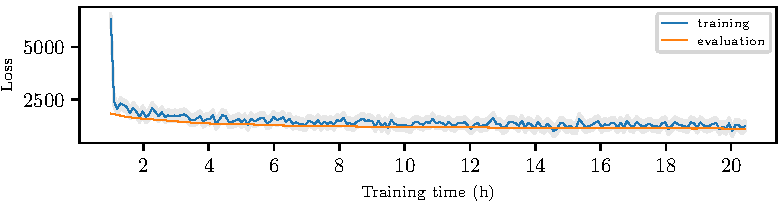
\includegraphics{figure/loss_plots/loss_plot_1a.pdf}
		\caption{Loss plot for the experiment 1a from Table \ref{table.eval.learning-rate} with learning rate $\eta=10^{-3}$.}
		\label{fig.loss-plot.1a}
	\end{figure}

	\vfill

	\begin{figure}[H]
		\centering
		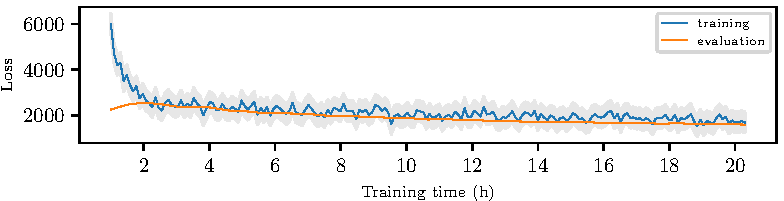
\includegraphics{figure/loss_plots/loss_plot_0.pdf}
		\caption{Loss plot for the experiment 0 from Table \ref{table.eval.baseline} with learning rate $\eta=10^{-5}$.}
		\label{fig.loss-plot.0}
	\end{figure}

	\vfill

	\pagebreak

	\begin{figure}[H]
		\centering
		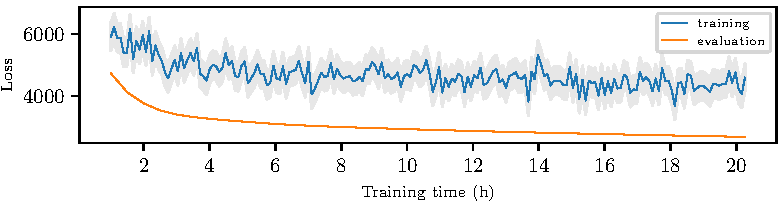
\includegraphics{figure/loss_plots/loss_plot_1c.pdf}
		\caption{Loss plot for the experiment 1c from Table \ref{table.eval.learning-rate} with learning rate $\eta=10^{-7}$.}
		\label{fig.loss-plot.1c}
	\end{figure}

	Furthermore, a higher batch size of $b_s=64$ leads to a smoother graph and lower loss compared to a batch size of $b_s=16$.

	\begin{figure}[H]
		\centering
		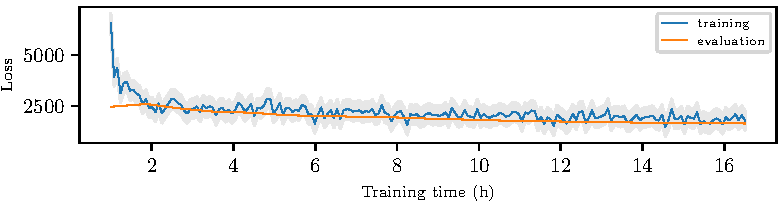
\includegraphics{figure/loss_plots/loss_plot_3b.pdf}
		\caption{Loss plot for the experiment 3b from Table \ref{table.eval.batch-size} with batch size $b_s=64$.}
		\label{fig.loss-plot.3b}
	\end{figure}

	\begin{figure}[H]
		\centering
		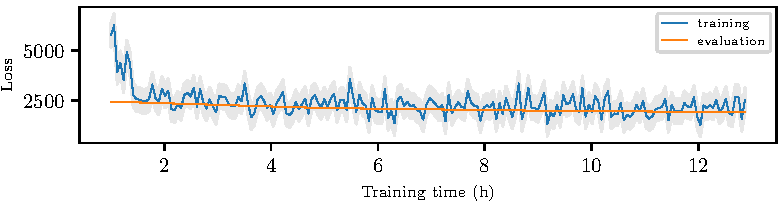
\includegraphics{figure/loss_plots/loss_plot_3d.pdf}
		\caption{Loss plot for the experiment 3d from Table \ref{table.eval.batch-size} with batch size $b_s=16$.}
		\label{fig.loss-plot.3d}
	\end{figure}
\end{appendices}

\cleardoublepage
\addcontentsline{toc}{chapter}{List of Figures}
\listoffigures

\cleardoublepage
\addcontentsline{toc}{chapter}{References}
\emergencystretch=1em
\printbibliography[title=References]

\end{document}
